% Options for packages loaded elsewhere
\PassOptionsToPackage{unicode}{hyperref}
\PassOptionsToPackage{hyphens}{url}
%
\documentclass[
]{book}
\usepackage{amsmath,amssymb}
\usepackage{iftex}
\ifPDFTeX
  \usepackage[T1]{fontenc}
  \usepackage[utf8]{inputenc}
  \usepackage{textcomp} % provide euro and other symbols
\else % if luatex or xetex
  \usepackage{unicode-math} % this also loads fontspec
  \defaultfontfeatures{Scale=MatchLowercase}
  \defaultfontfeatures[\rmfamily]{Ligatures=TeX,Scale=1}
\fi
\usepackage{lmodern}
\ifPDFTeX\else
  % xetex/luatex font selection
\fi
% Use upquote if available, for straight quotes in verbatim environments
\IfFileExists{upquote.sty}{\usepackage{upquote}}{}
\IfFileExists{microtype.sty}{% use microtype if available
  \usepackage[]{microtype}
  \UseMicrotypeSet[protrusion]{basicmath} % disable protrusion for tt fonts
}{}
\makeatletter
\@ifundefined{KOMAClassName}{% if non-KOMA class
  \IfFileExists{parskip.sty}{%
    \usepackage{parskip}
  }{% else
    \setlength{\parindent}{0pt}
    \setlength{\parskip}{6pt plus 2pt minus 1pt}}
}{% if KOMA class
  \KOMAoptions{parskip=half}}
\makeatother
\usepackage{xcolor}
\usepackage{color}
\usepackage{fancyvrb}
\newcommand{\VerbBar}{|}
\newcommand{\VERB}{\Verb[commandchars=\\\{\}]}
\DefineVerbatimEnvironment{Highlighting}{Verbatim}{commandchars=\\\{\}}
% Add ',fontsize=\small' for more characters per line
\usepackage{framed}
\definecolor{shadecolor}{RGB}{248,248,248}
\newenvironment{Shaded}{\begin{snugshade}}{\end{snugshade}}
\newcommand{\AlertTok}[1]{\textcolor[rgb]{0.94,0.16,0.16}{#1}}
\newcommand{\AnnotationTok}[1]{\textcolor[rgb]{0.56,0.35,0.01}{\textbf{\textit{#1}}}}
\newcommand{\AttributeTok}[1]{\textcolor[rgb]{0.13,0.29,0.53}{#1}}
\newcommand{\BaseNTok}[1]{\textcolor[rgb]{0.00,0.00,0.81}{#1}}
\newcommand{\BuiltInTok}[1]{#1}
\newcommand{\CharTok}[1]{\textcolor[rgb]{0.31,0.60,0.02}{#1}}
\newcommand{\CommentTok}[1]{\textcolor[rgb]{0.56,0.35,0.01}{\textit{#1}}}
\newcommand{\CommentVarTok}[1]{\textcolor[rgb]{0.56,0.35,0.01}{\textbf{\textit{#1}}}}
\newcommand{\ConstantTok}[1]{\textcolor[rgb]{0.56,0.35,0.01}{#1}}
\newcommand{\ControlFlowTok}[1]{\textcolor[rgb]{0.13,0.29,0.53}{\textbf{#1}}}
\newcommand{\DataTypeTok}[1]{\textcolor[rgb]{0.13,0.29,0.53}{#1}}
\newcommand{\DecValTok}[1]{\textcolor[rgb]{0.00,0.00,0.81}{#1}}
\newcommand{\DocumentationTok}[1]{\textcolor[rgb]{0.56,0.35,0.01}{\textbf{\textit{#1}}}}
\newcommand{\ErrorTok}[1]{\textcolor[rgb]{0.64,0.00,0.00}{\textbf{#1}}}
\newcommand{\ExtensionTok}[1]{#1}
\newcommand{\FloatTok}[1]{\textcolor[rgb]{0.00,0.00,0.81}{#1}}
\newcommand{\FunctionTok}[1]{\textcolor[rgb]{0.13,0.29,0.53}{\textbf{#1}}}
\newcommand{\ImportTok}[1]{#1}
\newcommand{\InformationTok}[1]{\textcolor[rgb]{0.56,0.35,0.01}{\textbf{\textit{#1}}}}
\newcommand{\KeywordTok}[1]{\textcolor[rgb]{0.13,0.29,0.53}{\textbf{#1}}}
\newcommand{\NormalTok}[1]{#1}
\newcommand{\OperatorTok}[1]{\textcolor[rgb]{0.81,0.36,0.00}{\textbf{#1}}}
\newcommand{\OtherTok}[1]{\textcolor[rgb]{0.56,0.35,0.01}{#1}}
\newcommand{\PreprocessorTok}[1]{\textcolor[rgb]{0.56,0.35,0.01}{\textit{#1}}}
\newcommand{\RegionMarkerTok}[1]{#1}
\newcommand{\SpecialCharTok}[1]{\textcolor[rgb]{0.81,0.36,0.00}{\textbf{#1}}}
\newcommand{\SpecialStringTok}[1]{\textcolor[rgb]{0.31,0.60,0.02}{#1}}
\newcommand{\StringTok}[1]{\textcolor[rgb]{0.31,0.60,0.02}{#1}}
\newcommand{\VariableTok}[1]{\textcolor[rgb]{0.00,0.00,0.00}{#1}}
\newcommand{\VerbatimStringTok}[1]{\textcolor[rgb]{0.31,0.60,0.02}{#1}}
\newcommand{\WarningTok}[1]{\textcolor[rgb]{0.56,0.35,0.01}{\textbf{\textit{#1}}}}
\usepackage{longtable,booktabs,array}
\usepackage{calc} % for calculating minipage widths
% Correct order of tables after \paragraph or \subparagraph
\usepackage{etoolbox}
\makeatletter
\patchcmd\longtable{\par}{\if@noskipsec\mbox{}\fi\par}{}{}
\makeatother
% Allow footnotes in longtable head/foot
\IfFileExists{footnotehyper.sty}{\usepackage{footnotehyper}}{\usepackage{footnote}}
\makesavenoteenv{longtable}
\usepackage{graphicx}
\makeatletter
\def\maxwidth{\ifdim\Gin@nat@width>\linewidth\linewidth\else\Gin@nat@width\fi}
\def\maxheight{\ifdim\Gin@nat@height>\textheight\textheight\else\Gin@nat@height\fi}
\makeatother
% Scale images if necessary, so that they will not overflow the page
% margins by default, and it is still possible to overwrite the defaults
% using explicit options in \includegraphics[width, height, ...]{}
\setkeys{Gin}{width=\maxwidth,height=\maxheight,keepaspectratio}
% Set default figure placement to htbp
\makeatletter
\def\fps@figure{htbp}
\makeatother
\ifLuaTeX
  \usepackage{luacolor}
  \usepackage[soul]{lua-ul}
\else
  \usepackage{soul}
\fi
\setlength{\emergencystretch}{3em} % prevent overfull lines
\providecommand{\tightlist}{%
  \setlength{\itemsep}{0pt}\setlength{\parskip}{0pt}}
\setcounter{secnumdepth}{5}
\usepackage{booktabs}
\usepackage{amssymb}
\usepackage{amsmath}
\usepackage{graphicx}
\usepackage{wasysym}
\usepackage{amsthm}
\usepackage{multirow}
\usepackage{epsf}
\usepackage{tikz}
\usepackage{cancel}
\usepackage{hyperref}
\usepackage{gensymb}
\usepackage{color}
\usepackage{framed}
\setlength{\fboxsep}{.8em}
\newenvironment{blackbox}{
  \definecolor{shadecolor}{rgb}{0, 0, 0}
  \color{white}
  \begin{shaded}
  }
 {\end{shaded}}
\ifLuaTeX
  \usepackage{selnolig}  % disable illegal ligatures
\fi
\usepackage[]{natbib}
\bibliographystyle{plainnat}
\usepackage{bookmark}
\IfFileExists{xurl.sty}{\usepackage{xurl}}{} % add URL line breaks if available
\urlstyle{same}
\hypersetup{
  pdftitle={Bookdown: Flexible Document Creation in RStudio},
  pdfauthor={Joseph Thiers},
  hidelinks,
  pdfcreator={LaTeX via pandoc}}

\title{Bookdown: Flexible Document Creation in RStudio}
\author{Joseph Thiers}
\date{}

\usepackage{amsthm}
\newtheorem{theorem}{Theorem}[chapter]
\newtheorem{lemma}{Lemma}[chapter]
\newtheorem{corollary}{Corollary}[chapter]
\newtheorem{proposition}{Proposition}[chapter]
\newtheorem{conjecture}{Conjecture}[chapter]
\theoremstyle{definition}
\newtheorem{definition}{Definition}[chapter]
\theoremstyle{definition}
\newtheorem{example}{Example}[chapter]
\theoremstyle{definition}
\newtheorem{exercise}{Exercise}[chapter]
\theoremstyle{definition}
\newtheorem{hypothesis}{Hypothesis}[chapter]
\theoremstyle{remark}
\newtheorem*{remark}{Remark}
\newtheorem*{solution}{Solution}
\begin{document}
\maketitle

{
\setcounter{tocdepth}{1}
\tableofcontents
}
\chapter{Introduction to Bookdown}\label{introduction}

In today's fast-paced academic and professional environments, the ability to create dynamic, reproducible documents is crucial. Bookdown empowers users to combine text, code, and visualizations in a single, streamlined workflow. It is ideal for creating the type of documentation that best fits your needs, whether that be single-page assignments, reports, academic papers, or even full-length books.

\section{Why RStudio and Bookdown?}\label{why-rstudio-and-bookdown}

Bookdown offers a range of benefits:

\begin{itemize}
\item
  Seamlessly integrates text, code, and figures.
\item
  Supports multiple output formats (HTML, PDF, EPUB).
\item
  Simplifies the creation of reproducible and professional documents.
\item
  Ideal for mathematics, statistics, and data science professionals.
\end{itemize}

\section{Robust Documentation and Support}\label{robust-documentation-and-support}

\begin{itemize}
\item
  Bookdown Documentation \url{https://bookdown.org/yihui/bookdown/}
\item
  R Markdown Cookbook \url{https://bookdown.org/yihui/rmarkdown-cookbook/}
\item
  Pandoc \url{https://pandoc.org/}
\item
  RStudio Bookdown Community \url{https://community.rstudio.com/tags/bookdown}
\item
  Gallery of Books you can Download \url{https://bookdown.org/home/archive/}
\end{itemize}

\section{What You'll Learn in This Tutorial}\label{what-youll-learn-in-this-tutorial}

This tutorial will guide you through the essential aspects of using Bookdown:

\begin{itemize}
\tightlist
\item
  \textbf{Chapter \ref{introduction}}: Introduction to Bookdown -- Learn about its purpose and benefits for structured documentation.
\item
  \textbf{Chapter \ref{chapter2}}: Getting Started -- Install R, RStudio, and Bookdown, create a project, and render your first book.
\item
  \textbf{Chapter \ref{chapter3}}: Writing Content -- Organize chapters, use Markdown, format text, add code chunks, and images.
\item
  \textbf{Chapter \ref{chapter4}}: Cross-Referencing -- Reference sections, figures, tables, and equations effectively.
\item
  \textbf{Chapter \ref{chapter5}}: LaTeX -- Add equations, theorems, lemmas, and proofs.
\item
  \textbf{Chapter \ref{chapter6}}: Advanced Features -- Manage citations, use LaTeX packages, and more!
\item
  \textbf{Chapter \ref{chapter7}}: Customizing Output -- Configure formats like HTML, PDF, and EPUB, and style your book with CSS or LaTeX.
\item
  \textbf{Chapter \ref{latexdistributions}}: LaTeX Distributions - Different distributions available.
\item
  \textbf{Chapter \ref{markdownadvanced}}: Advanced Text Formatting Options - Advanced Markdown and Pandoc code to stylize the book to your needs.
\item
  \textbf{Chapter \ref{examplepaper}}: Example Document: Union Earnings Analysis
\end{itemize}

By the end of this tutorial, you'll have the knowledge to create, customize, and publish professional-grade documents.

\chapter{Getting Started}\label{chapter2}

To get started with Bookdown you need to install R, RStudio, Bookdown, and the LaTeX distribution of your choice if you wish to output as a PDF. This can be accomplished by following these steps::

\begin{enumerate}
\def\labelenumi{\arabic{enumi}.}
\tightlist
\item
  \textbf{Install R}
  Go to the \href{https://cran.r-project.org/}{R Project download page} and download the latest version of R for your operating system (Windows, macOS, or Linux). Follow the installation instructions provided.
\end{enumerate}


\includegraphics[width=27.33in]{images/tutorialscreenshots/installR}

\begin{enumerate}
\def\labelenumi{\arabic{enumi}.}
\setcounter{enumi}{1}
\item
  \textbf{Install RStudio}:\\
  Go to the \href{https://posit.co/download/rstudio-desktop/}{RStudio download page} and select the appropriate version for your operating system. Download and follow the installation instructions.

  
\includegraphics[width=16.83in]{images/tutorialscreenshots/installRStudio}
\item
  \textbf{Install Bookdown}:\\
  Once RStudio is installed, install the Bookdown package by typing the following command in the RStudio console:

\begin{Shaded}
\begin{Highlighting}[]
\FunctionTok{install.packages}\NormalTok{(}\StringTok{"bookdown"}\NormalTok{)}
\end{Highlighting}
\end{Shaded}

  Alternatively, you can install the Bookdown package via the RStudio \textbf{Packages} pane:

  \begin{itemize}
  \item
    Select \textbf{Packages} in the bottom right-hand corner of RStudio.

    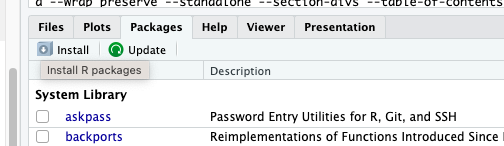
\includegraphics[width=7in]{images/tutorialscreenshots/installPackage}
  \item
    Click \textbf{Install}, type \texttt{bookdown} in the \textbf{Packages} box, and click \textbf{Install}.

    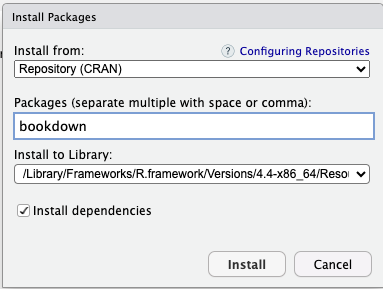
\includegraphics[width=5.32in]{images/tutorialscreenshots/installBookdownPack}
  \end{itemize}
\item
  \textbf{Install LaTeX distribution of your choice}:
  The distribution you choose is entirely up to you and your needs. For a list of recommended LaTeX distributions please see \hyperref[latexdistributions]{LaTeX Distributions Chapter \ref{latexdistributions}}
\end{enumerate}

To get started quickly TinyTeX is recommended as it can be installed from within RStudio by running the following code:

\begin{verbatim}
install.packages("tinytex")
tinytex::install_tinytex()
\end{verbatim}

Once this is complete Bookdown is now installed and you are ready to create your first Bookdown project.

\begin{enumerate}
\def\labelenumi{\arabic{enumi}.}
\setcounter{enumi}{4}
\tightlist
\item
  \textbf{Create a New Bookdown Project in RStudio}:

  \begin{itemize}
  \tightlist
  \item
    In RStudio, go to \textbf{File \textgreater{} New Project}.
  \item
    Select \textbf{New Directory} and then \textbf{Book Project using Bookdown}.
  \item
    Name your project and choose a location to save it to.
  \end{itemize}
\end{enumerate}

Now you have a newly created Bookdown project ready to be edited to fit your needs. Bookdown comes with a base set of files so that users can get started quickly with minimal fuss. Spend a few moments to explore the files in the bottom right corner of RStudio, these are the default files Bookdown creates to get you started. It even includes sample chapters for you!

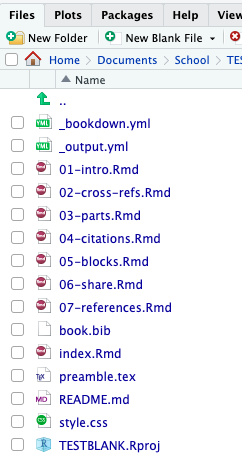
\includegraphics[width=3.36in]{images/tutorialscreenshots/filestructure}

Let's go over quickly what you're seeing.

\texttt{\_bookdown.yml} This file controls the settings for your Bookdown project, such as the order of the chapters and output options.

\texttt{\_output.yml} This file specifics the formats your book will be rendered into, such as PDF, HTML, or Word.

\texttt{index.Rmd} Is the main file where your book starts. This page contains the title, author, and any other introductory information you may want your readers to know.

\texttt{01-intro.Rmd}, \texttt{02-cross-regs.Rmd}, \texttt{03-parts.Rmd}, \texttt{04-citations.Rmd}, \texttt{05-blocks.Rmd}, \texttt{06-share.Rmd} and \texttt{07-references.Rmd} are all sample chapters that the initial bookdown project creates for you. Starting from 01-07 these are the chapters after your Introduction and you can have as many as you want, or even just a single chapter. This way you have handy easy to edit chapters ready for you to edit, simplifying the work you need to get started.

\texttt{book.bib} is the reference file you place all your references you may need to cite in your book.

\texttt{preamble.tex} is where you enter any packages you may wish to use for your LaTeX entries.

\texttt{style.css} is where you will enter any custom CSS you may want to use to customize the look of your book in html.

When you're ready to complete your project just follow the last step below to render your book.

\begin{enumerate}
\def\labelenumi{\arabic{enumi}.}
\setcounter{enumi}{5}
\tightlist
\item
  \textbf{Render Your Newly Created Book}:\\
  In the \textbf{Build} pane:

  \begin{itemize}
  \tightlist
  \item
    Select \textbf{Build Book} and choose your output format, or select \emph{All formats} to render your files as HTML, PDF, and EPUB.
  \item
    You can also render the book directly from the R console with the following command:
  \end{itemize}

\begin{Shaded}
\begin{Highlighting}[]
\NormalTok{bookdown}\SpecialCharTok{::}\FunctionTok{render\_book}\NormalTok{(}\StringTok{"index.Rmd"}\NormalTok{)}
\end{Highlighting}
\end{Shaded}
\end{enumerate}

\chapter{Writing Content}\label{chapter3}

In this chapter, we will explore how to write and structure content in Bookdown using R Markdown syntax. Bookdown allows you to create well-organized documents by combining text, code, and references. Here, we'll cover how to organize chapters, use Markdown and LaTeX for formatting, and format text, code chunks, and images.

\begin{center}\rule{0.5\linewidth}{0.5pt}\end{center}

\section{Creating Chapters and Sections}\label{creating-chapters-and-sections}

Each chapter in Bookdown is represented by a separate \texttt{.Rmd} file, and each \texttt{.Rmd} file should begin with a first-level heading, marked by a single \texttt{\#} symbol. For example, this chapter file is \texttt{02-writing-content.Rmd} and the file starts with:

\begin{Shaded}
\begin{Highlighting}[]
\FunctionTok{\# Writing Content}
\end{Highlighting}
\end{Shaded}

\subsection{Organizing Chapters}\label{organizing-chapters}

Chapters are automatically numbered based on their order in the project directory. Ensure that each file name reflects its chapter number (e.g., \texttt{02-writing-content.Rmd} for Chapter 2). So if you need to add new chapters to your book just make sure you adjust the filename of any other chapters you already have to ensure it fits. For example, if you need to add a new chapter between 3 and 4, you would need to make sure that you rename your chpater 4 file from 03 to 04, and your new file would start with 03.

\subsection{Adding Sections and Subsections}\label{adding-sections-and-subsections}

You can add sections and subsections within a chapter using second-level and higher-level headings:

\begin{Shaded}
\begin{Highlighting}[]
\FunctionTok{\#\# Section Title}
\FunctionTok{\#\#\# Subsection Title}
\end{Highlighting}
\end{Shaded}

This hierarchy organizes the document according to your needs, and these sections will automatically appear in the table of contents.

\begin{center}\rule{0.5\linewidth}{0.5pt}\end{center}

\section{Formatting Text in Bookdown}\label{formatting-text-in-bookdown}

Bookdown supports a wide range of Markdown formatting. Here are a few basics:

\begin{itemize}
\tightlist
\item
  \textbf{Bold}: \texttt{**bold\ text**} → \textbf{bold text}
\item
  \emph{Italics}: \texttt{*italicized\ text*} → \emph{italicized text}
\item
  \textbf{Bullet Points}:

  \begin{itemize}
  \tightlist
  \item
    First item
  \item
    Second item
  \end{itemize}
\item
  \textbf{Numbered Lists}:

  \begin{enumerate}
  \def\labelenumi{\arabic{enumi}.}
  \tightlist
  \item
    First item

    \begin{itemize}
    \tightlist
    \item
      Even sublists
    \item
      Like this
    \end{itemize}
  \item
    Second item
  \end{enumerate}
\end{itemize}

\subsection{Creating Tables in Bookdown}\label{creating-tables-in-bookdown}

Tables are a powerful way to organize and present data in Bookdown. You can create tables using basic Markdown syntax.

\section{Creating Basic Markdown Tables}\label{creating-basic-markdown-tables}

It's quite easy to create your own table as well. All you need to do is format it as such:

\begin{Shaded}
\begin{Highlighting}[]
\PreprocessorTok{|}\NormalTok{ Column 1     }\PreprocessorTok{|}\NormalTok{ Column 2     }\PreprocessorTok{|}\NormalTok{ Column 3     }\PreprocessorTok{|}
\PreprocessorTok{|{-}{-}{-}{-}{-}{-}{-}{-}{-}{-}{-}{-}{-}{-}|{-}{-}{-}{-}{-}{-}{-}{-}{-}{-}{-}{-}{-}{-}|{-}{-}{-}{-}{-}{-}{-}{-}{-}{-}{-}{-}{-}{-}|}
\PreprocessorTok{|}\NormalTok{ Row 1, Col 1 }\PreprocessorTok{|}\NormalTok{ Row 1, Col 2 }\PreprocessorTok{|}\NormalTok{ Row 1, Col 3 }\PreprocessorTok{|}
\PreprocessorTok{|}\NormalTok{ Row 2, Col 1 }\PreprocessorTok{|}\NormalTok{ Row 2, Col 2 }\PreprocessorTok{|}\NormalTok{ Row 2, Col 3 }\PreprocessorTok{|}
\end{Highlighting}
\end{Shaded}

This will then be outputted as:

\begin{longtable}[]{@{}lll@{}}
\toprule\noalign{}
Column 1 & Column 2 & Column 3 \\
\midrule\noalign{}
\endhead
\bottomrule\noalign{}
\endlastfoot
Row 1, Col 1 & Row 1, Col 2 & Row 1, Col 3 \\
Row 2, Col 1 & Row 2, Col 2 & Row 2, Col 3 \\
\end{longtable}

For additional text formatting options refer to \hyperref[markdown-advanced]{Chapter 9 Advanced Text Formatting}.

Use these formatting options to style text and create lists within your chapters.

\begin{center}\rule{0.5\linewidth}{0.5pt}\end{center}

\section{Adding Code Chunks}\label{adding-code-chunks}

One of the strengths of Bookdown is the ability to incorporate code into your document, whether it's R code, Markdown, LaTeX, Python, or other languages. Below are examples of how to include different types of code in your Bookdown project.

\subsection{Example: Loading Data}\label{example-loading-data}

To include R code chunks in your Bookdown project, use three backticks \texttt{\textasciigrave{}\textasciigrave{}\textasciigrave{}} with \texttt{\{r\}} specifying the language. For other languages you would just change r to the language of your choice such as Python or Java. For example say you want to show users how you set a working directory for your data analysis on Union Wages, you could do it as follows:

\begin{verbatim}
{r eval=FALSE, warning=FALSE, include=TRUE, results='hide'}
# Set the working directory and load data files
setwd("~/Documents/School/RaceIncomeCalifornia")
demographics <- readr::read_csv('demographics.csv')
wages <- readr::read_csv('wages.csv')
states <- readr::read_csv('states.csv')
\end{verbatim}

In this example, the \texttt{eval=FALSE} option prevents the code from being executed during rendering, while the \texttt{warning=FALSE} and \texttt{include=TRUE} options suppress warnings and ensure the chunk is included in the output.

\subsection{Customizing Code Chunk Options}\label{customizing-code-chunk-options}

Use chunk options to control how the code and output appear in the document. Here is a short list of different code chunk options that you have as a user. All code chunk options are formatted with an equal sign after them, before TRUE, FALSE, or other option, when adding them to your code chunk as such: \texttt{eval=TRUE} or \texttt{fig.align=\textquotesingle{}center\textquotesingle{}}. Here is a list of some basic and handy code chunk options to get you started.

Basic Options

\begin{longtable}[]{@{}
  >{\raggedright\arraybackslash}p{(\columnwidth - 2\tabcolsep) * \real{0.1613}}
  >{\raggedright\arraybackslash}p{(\columnwidth - 2\tabcolsep) * \real{0.8387}}@{}}
\toprule\noalign{}
\begin{minipage}[b]{\linewidth}\raggedright
\textbf{Option}
\end{minipage} & \begin{minipage}[b]{\linewidth}\raggedright
\textbf{Description}
\end{minipage} \\
\midrule\noalign{}
\endhead
\bottomrule\noalign{}
\endlastfoot
\texttt{eval} & Executes the code if \texttt{TRUE} (default); skips execution if \texttt{FALSE}. \\
\texttt{echo} & Displays the code in the output if \texttt{TRUE} (default); hides code if \texttt{FALSE}. \\
\texttt{results} & Determines how results are displayed (\texttt{"markup"}, \texttt{"asis"}, \texttt{"hide"}). \\
\texttt{message} & Displays messages from the code if \texttt{TRUE} (default); hides them if \texttt{FALSE}. \\
\texttt{warning} & Displays warnings if \texttt{TRUE} (default); suppresses them if \texttt{FALSE}. \\
\texttt{error} & Displays error messages if \texttt{TRUE}; suppresses them if \texttt{FALSE}. \\
\end{longtable}

\begin{center}\rule{0.5\linewidth}{0.5pt}\end{center}

Output Control

\begin{longtable}[]{@{}
  >{\raggedright\arraybackslash}p{(\columnwidth - 2\tabcolsep) * \real{0.1848}}
  >{\raggedright\arraybackslash}p{(\columnwidth - 2\tabcolsep) * \real{0.8152}}@{}}
\toprule\noalign{}
\begin{minipage}[b]{\linewidth}\raggedright
\textbf{Option}
\end{minipage} & \begin{minipage}[b]{\linewidth}\raggedright
\textbf{Description}
\end{minipage} \\
\midrule\noalign{}
\endhead
\bottomrule\noalign{}
\endlastfoot
\texttt{fig.width} & Width of the generated figure (in inches). \\
\texttt{fig.height} & Height of the generated figure (in inches). \\
\texttt{fig.align} & Aligns the figure (\texttt{"left"}, \texttt{"right"}, \texttt{"center"}). \\
\texttt{fig.cap} & Adds a caption to the figure (e.g., \texttt{fig.cap="Figure\ caption"}). \\
\texttt{out.width} & Width of the figure output (e.g., \texttt{out.width="50\%"}). \\
\texttt{out.height} & Height of the figure output (similar to \texttt{out.width}). \\
\texttt{fig.show} & Controls figure display (\texttt{"asis"}, \texttt{"hold"}, \texttt{"hide"}). \\
\end{longtable}

As an example say you need to run some behind the scenes data manipulation of what you've downloaded so that you can do an analysis and plot later on in your document. You could set your code chunk options so that it runs but is hidden by setting \texttt{eval=TRUE} so that it executes the code, \texttt{echo=FALSE} to not display the code, then \texttt{results=hide}, \texttt{warning=FALSE}, and \texttt{message=FALSE} to prevent any results or possible warning messages from appear in your code.

\begin{verbatim}
{r, eval=TRUE, echo=FALSE, results='hide', warning=FALSE, message=FALSE}

setwd("~/Documents/School/RaceIncomeCalifornia")
demographics <- readr::read_csv('demographics.csv')
wages <- readr::read_csv('wages.csv')
states <- readr::read_csv('states.csv')

filtered_wages <- wages[wages$year >= 2000, ]
filtered_states <- states[states$year >= 2000, ]
filtered_demographics <- demographics[demographics$year >= 2000, ]

merged_data <- merge(states, wages, by = "year", all.x = TRUE)


if (!requireNamespace("data.table", quietly = TRUE)) {
  install.packages("data.table")
}
library(data.table)

setDT(filtered_wages)
setDT(filtered_states)
setDT(filtered_demographics)

wage_trends <- filtered_wages[, 
      list(mean_union_wage = mean(union_wage, 
                                  na.rm = TRUE),
      mean_nonunion_wage = mean(nonunion_wage, 
                                na.rm = TRUE)), by = list(year)]

union_wage_premium <- filtered_wages[, 
      list(raw_premium = mean(union_wage_premium_raw, na.rm = TRUE),
      adjusted_premium = mean(union_wage_premium_adjusted, 
                              na.rm = TRUE)), by = year]

membership_trends <- filtered_demographics[, 
        list(average_p_members = mean(p_members, na.rm = TRUE)), by = year]

average_wage_by_year <- filtered_wages[,
      list(average_wage = (mean(union_wage, na.rm = TRUE) + 
      mean(nonunion_wage, na.rm = TRUE)) / 2), 
        by = list(year)]

merged_data$members_scaled <- merged_data$members * 100
\end{verbatim}

When rendered, this chunk will execute in the background, ensuring the data is processed, but no code, output, warnings, or messages will be visible in your final document, this way you can ensure it gets run every time your book is outputted.

\begin{center}\rule{0.5\linewidth}{0.5pt}\end{center}

\section{Adding Plots and Images to Your Bookdown Project}\label{adding-plots-and-images-to-your-bookdown-project}

Plots and images can enhance your document by providing visual context. In Bookdown, you can add plots using R code, use Markdown or by embedding images using R code chunks.

\subsection{Adding Images with RStudio GGPLOT}\label{adding-images-with-rstudio-ggplot}

The easiest way to add images more relevant to your needs is with the built in plotting functions of RStudio, or the ggplot package. Simply add an R code chunk and enter the code you wish to run. For example, say you you want to show a plot showing the wage increases for Union Members compared to non-Union members.

\begin{Shaded}
\begin{Highlighting}[]
\FunctionTok{ggplot}\NormalTok{(wages, }\FunctionTok{aes}\NormalTok{(}\AttributeTok{x =}\NormalTok{ year)) }\SpecialCharTok{+}
  \FunctionTok{geom\_smooth}\NormalTok{(}\FunctionTok{aes}\NormalTok{(}\AttributeTok{y =}\NormalTok{ union\_wage, }\AttributeTok{color =} \StringTok{"Union Wage"}\NormalTok{), }
              \AttributeTok{se =} \ConstantTok{FALSE}\NormalTok{, }\AttributeTok{method =} \StringTok{"loess"}\NormalTok{) }\SpecialCharTok{+}
  \FunctionTok{geom\_smooth}\NormalTok{(}\FunctionTok{aes}\NormalTok{(}\AttributeTok{y =}\NormalTok{ nonunion\_wage, }\AttributeTok{color =} \StringTok{"Nonunion Wage"}\NormalTok{), }
              \AttributeTok{se =} \ConstantTok{FALSE}\NormalTok{, }\AttributeTok{method =} \StringTok{"loess"}\NormalTok{) }\SpecialCharTok{+}
  \FunctionTok{labs}\NormalTok{(}\AttributeTok{x =} \StringTok{"Year"}\NormalTok{, }\AttributeTok{y =} \StringTok{"Wage"}\NormalTok{,}
       \AttributeTok{color =} \StringTok{"Type of Wage"}\NormalTok{) }\SpecialCharTok{+}
  \FunctionTok{theme\_minimal}\NormalTok{(}\AttributeTok{base\_size =} \DecValTok{14}\NormalTok{) }\SpecialCharTok{+}
  \FunctionTok{theme}\NormalTok{(}\AttributeTok{legend.position =} \StringTok{"bottom"}\NormalTok{) }\SpecialCharTok{+}
  \FunctionTok{scale\_color\_manual}\NormalTok{(}\AttributeTok{values =} \FunctionTok{c}\NormalTok{(}\StringTok{"Union Wage"} \OtherTok{=} \StringTok{"blue"}\NormalTok{, }\StringTok{"Nonunion Wage"} \OtherTok{=} \StringTok{"green"}\NormalTok{)) }\SpecialCharTok{+}
  \FunctionTok{guides}\NormalTok{(}\AttributeTok{color =} \FunctionTok{guide\_legend}\NormalTok{(}\AttributeTok{title =} \StringTok{"Wage Type"}\NormalTok{))}
\end{Highlighting}
\end{Shaded}

\begin{figure}
\centering
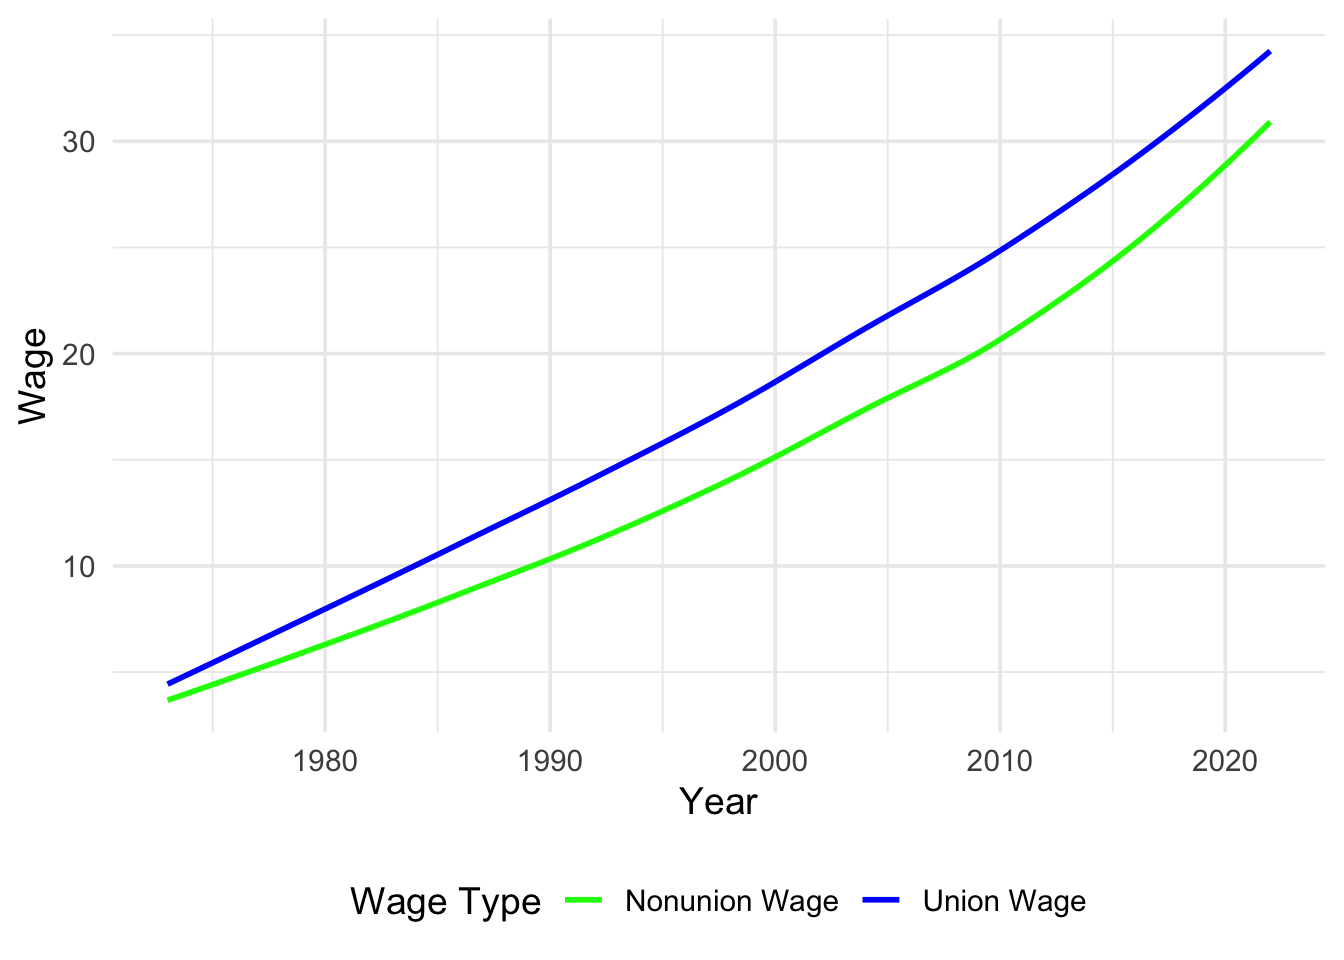
\includegraphics{_main_files/figure-latex/wagecomparison-1.pdf}
\caption{\label{fig:wagecomparison}Union Vs Non-Union Wages}
\end{figure}

As you can see the above code then creates a plot and places it in your document for you. This way you can fully customize the plot from within RStudio.

\subsection{Adding Images Using Markdown}\label{adding-images-using-markdown}

To add an image using Markdown, use the following syntax:

\begin{Shaded}
\begin{Highlighting}[]
\AlertTok{![Alt text for the image](images/wagesector.png)}
\end{Highlighting}
\end{Shaded}

\begin{itemize}
\tightlist
\item
  \textbf{Alt text}: A description of the image that is useful for accessibility.
\item
  \textbf{Path to the image}: This can be a relative path (e.g., \texttt{images/wagesector.png}) or a URL.
\end{itemize}

Example:

\begin{Shaded}
\begin{Highlighting}[]
\AlertTok{![A sample image](images/wagesector.png)}
\end{Highlighting}
\end{Shaded}

\begin{figure}
\centering
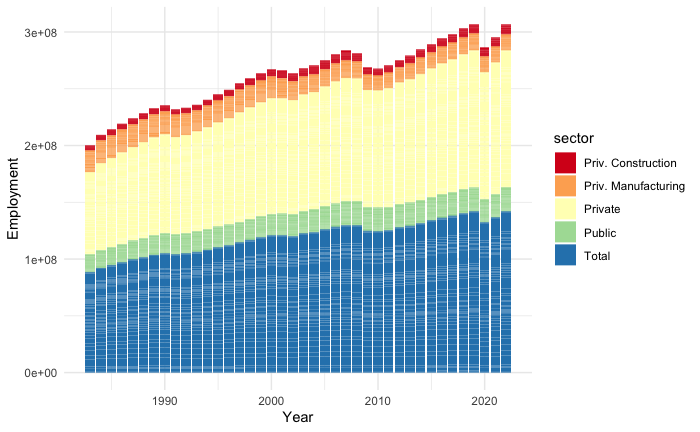
\includegraphics{images/wagesector.png}
\caption{A sample image}
\end{figure}

\subsection{Adding Images Using Code Chunks}\label{adding-images-using-code-chunks}

You can also add images using an R code chunk, which can be useful when the image is generated programmatically. Use the \texttt{knitr::include\_graphics()} function:

\begin{Shaded}
\begin{Highlighting}[]
\NormalTok{knitr}\SpecialCharTok{::}\FunctionTok{include\_graphics}\NormalTok{(}\StringTok{"images/wageyear{-}1.png"}\NormalTok{)}
\end{Highlighting}
\end{Shaded}

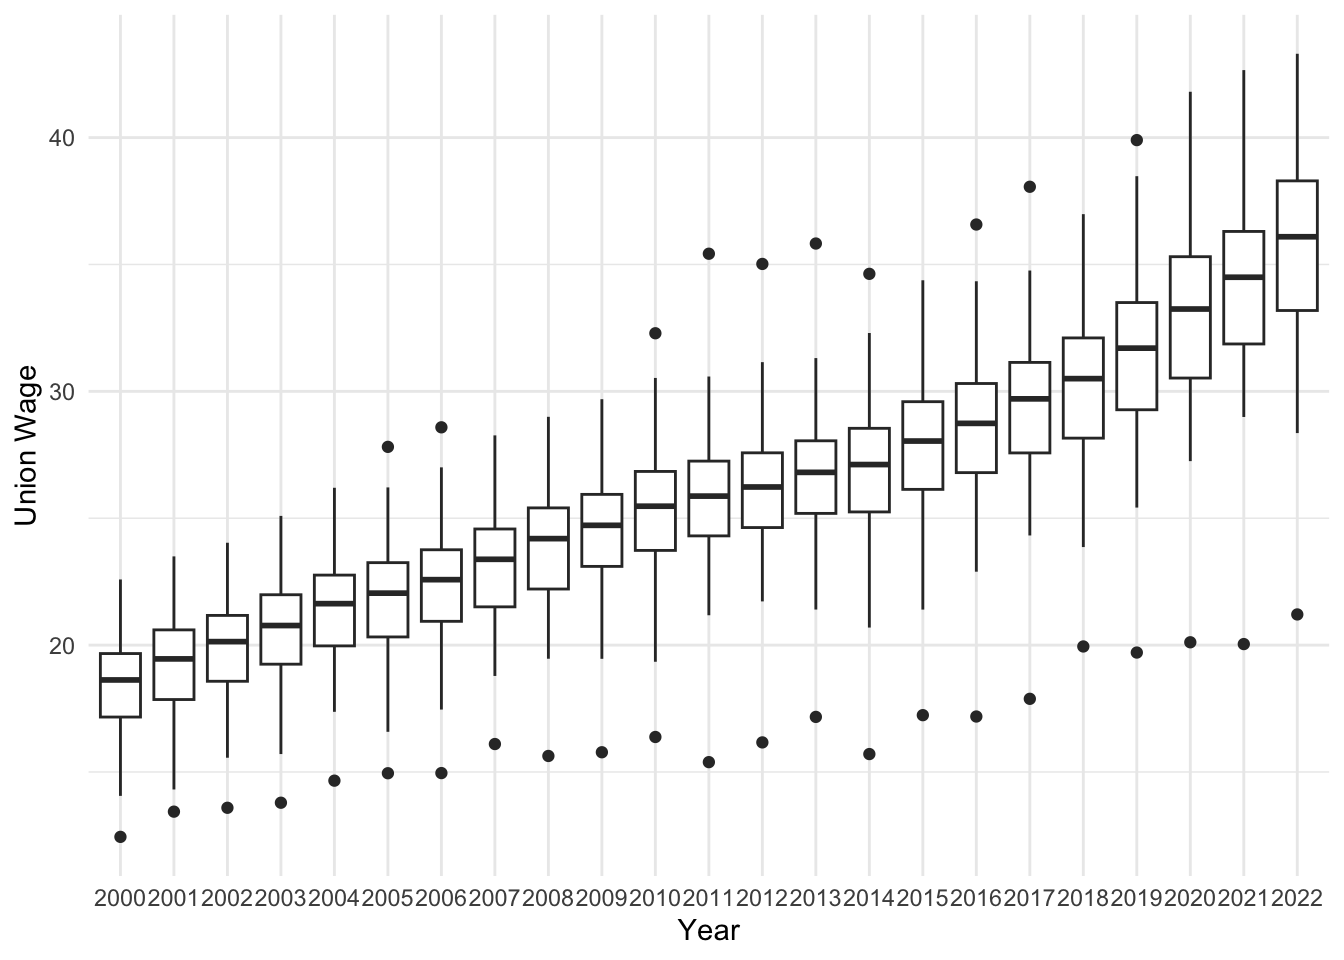
\includegraphics[width=18.67in]{images/wageyear-1}

\section{Chunk Options for Images}\label{chunk-options-for-images}

When adding images through code chunks, you can customize their appearance using chunk options such as \texttt{fig.cap} for captions and \texttt{out.width} for sizing.

For example the following has the caption \texttt{fig.cap="An\ example\ image"} and has an output width of 25\% with \texttt{out.width="25\%}. As you can see the image is much smaller than allowing the output width to not be adjusted.

\begin{Shaded}
\begin{Highlighting}[]
\NormalTok{knitr}\SpecialCharTok{::}\FunctionTok{include\_graphics}\NormalTok{(}\StringTok{"images/wageyear{-}1.png"}\NormalTok{)}
\end{Highlighting}
\end{Shaded}

\begin{figure}
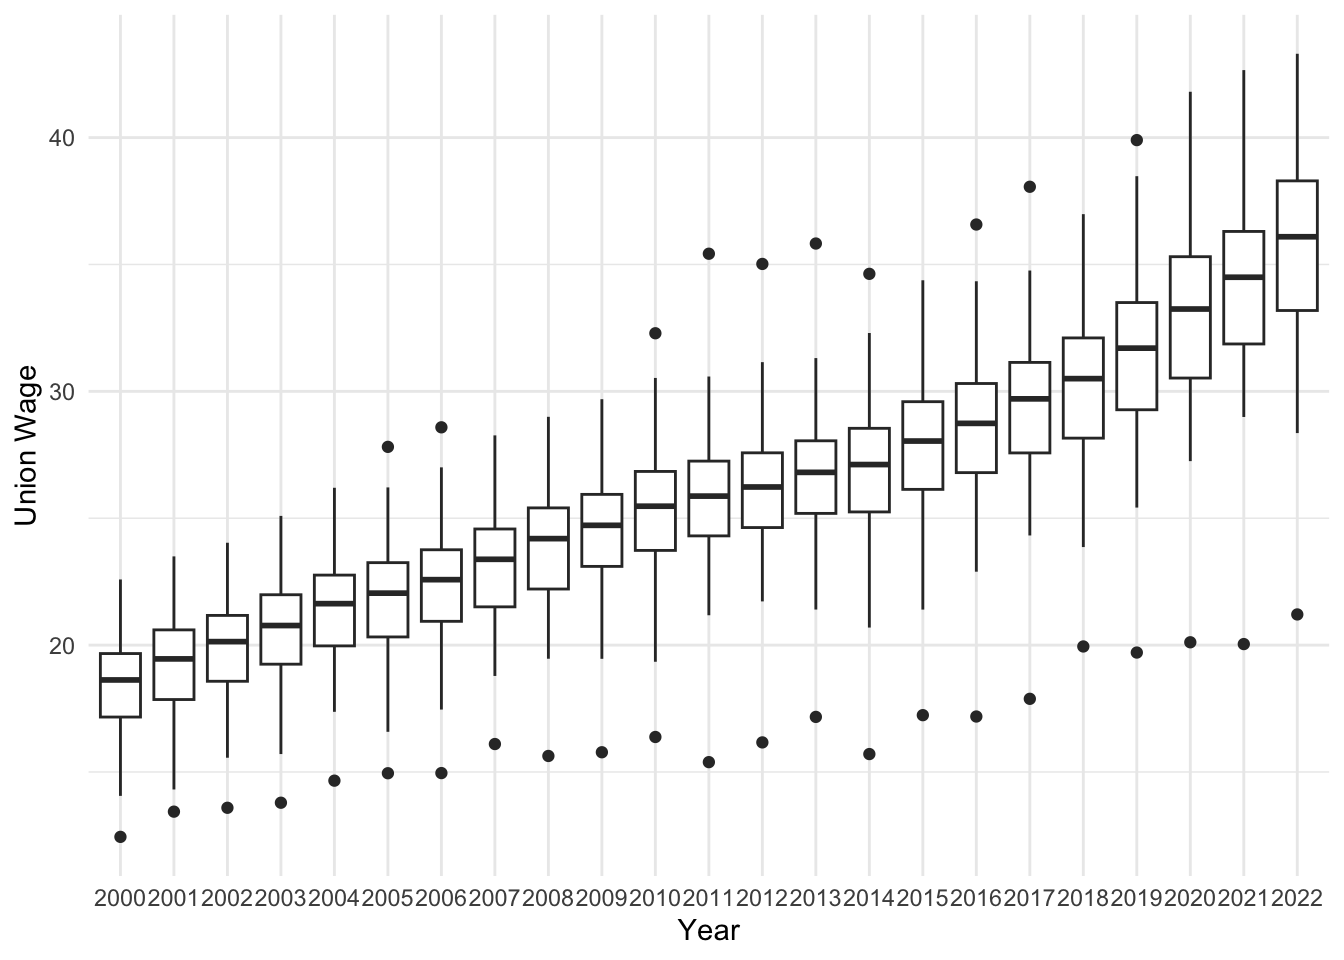
\includegraphics[width=0.25\linewidth]{images/wageyear-1} \caption{wageyear}\label{fig:unnamed-chunk-8}
\end{figure}

\begin{blackbox}

\begin{center}
\textbf{EXERCISE TIME!}

\end{center}

Create a new .Rmd file and write a short chapter that includes different types of Markdown elements (e.g., headers, tables, and images). Experiment with adding code chunks, and text formatting.

\end{blackbox}

\chapter{Cross Referencing and Citations}\label{chapter4}

Cross-references make it easier for readers to find and link to elements in your book. In Bookdown, you can create cross-references for sections, figures, tables, and equations. This chapter explains how to use cross-references effectively.

\begin{center}\rule{0.5\linewidth}{0.5pt}\end{center}

\section{Cross-Referencing Sections}\label{cross-referencing-sections}

To reference a section, first add an ID or tag to the heading by including \texttt{\{\#your-id\}} at the end of the section header. As an example here is the last chapter of the book that is an analysis I created within bookdown set as a single chapter:

\begin{Shaded}
\begin{Highlighting}[]
\FunctionTok{\# Example Document: Union Earnings Analysis (\#examplepaper)}
\end{Highlighting}
\end{Shaded}

You can then refer to it later, with a clickable link that will take your reader directly to it, in your document as follows:

\begin{Shaded}
\begin{Highlighting}[]
\NormalTok{See Section \textbackslash{}@ref(examplepaper) for more information.}
\end{Highlighting}
\end{Shaded}

\section{See Section \ref{examplepaper} for more information.}\label{see-section-refexamplepaper-for-more-information.}

\subsection{Cross-Referencing Text}\label{cross-referencing-text}

You can assign some text to a label and reference the text using the label elsewhere in your document. This can be particularly useful for long figure/table captions or when you need to reuse text fragments in multiple places.

The syntax for a text reference is \texttt{(ref:label)\ text}, where \texttt{label} is a unique label throughout the document. It must be in a separate paragraph with empty lines above and below it. The paragraph must not be wrapped into multiple lines, and should not end with whitespace.

\textbf{Additional Guidelines}:
- Ensure that text references are in a separate paragraph with empty lines above and below.
- Avoid wrapping the paragraph containing the text reference into multiple lines.
- Make sure there is no trailing whitespace at the end of the paragraph.

Example:

\begin{verbatim}



Then you can reference this text in your document using \texttt{(ref:textreference)}.

For example:

Then we reference it:
This is the text we are referencing
\end{verbatim}.

\begin{center}\rule{0.5\linewidth}{0.5pt}\end{center}

\subsection{Cross-Referencing Figures}\label{cross-referencing-figures}

To cross-reference a figure, set a chunk label and use the \texttt{fig.cap} option to add a caption. Bookdown automatically labels the figure with \texttt{fig:chunk-label}.

For example in the previous chapter we showed a plot comparing Union Wages vs Non-Union Wages. It had the following in the code chunk heading:

\texttt{\{r\ wagecomparison,\ fig.cap="Union\ Vs\ Non-Union\ Wages"\}}

We can easily create a reference back to this plot, that is clickable so users can easily go back to it, with the following:

\begin{Shaded}
\begin{Highlighting}[]
\NormalTok{See Figure \textbackslash{}@ref(fig:wagecomparison) for details.}
\end{Highlighting}
\end{Shaded}

See Figure \ref{fig:wagecomparison} for details.

\begin{center}\rule{0.5\linewidth}{0.5pt}\end{center}

\subsection{Cross-Referencing Tables}\label{cross-referencing-tables}

To cross-reference a table, use \texttt{knitr::kable()} to create a table with a caption. Bookdown automatically labels the table with \texttt{tab:chunk-label}.

Example:

\begin{Shaded}
\begin{Highlighting}[]
\NormalTok{knitr}\SpecialCharTok{::}\FunctionTok{kable}\NormalTok{(}\FunctionTok{head}\NormalTok{(cars), }\AttributeTok{caption =} \StringTok{"Table of the first rows of the cars dataset"}\NormalTok{)}
\end{Highlighting}
\end{Shaded}

\begin{table}

\caption{\label{tab:cars-table}Table of the first rows of the cars dataset}
\centering
\begin{tabular}[t]{r|r}
\hline
speed & dist\\
\hline
4 & 2\\
\hline
4 & 10\\
\hline
7 & 4\\
\hline
7 & 22\\
\hline
8 & 16\\
\hline
9 & 10\\
\hline
\end{tabular}
\end{table}

Reference this table using:

\begin{Shaded}
\begin{Highlighting}[]
\NormalTok{See Table \textbackslash{}@ref(tab:cars{-}table) for details.}
\end{Highlighting}
\end{Shaded}

See Table \ref{tab:cars-table} for details.

\begin{center}\rule{0.5\linewidth}{0.5pt}\end{center}

\section{Cross-Referencing Equations}\label{cross-referencing-equations}

For equations, use \texttt{(\textbackslash{}\#eq:label)} to label the equation and \texttt{\textbackslash{}@ref(eq:label)} to reference it. This way when you need to reference the equation at a later point in your document you can.

\subsection{Creating and Labeling an Equation}\label{creating-and-labeling-an-equation}

First you write the equation in LaTeX in the equation environment and include the label as \texttt{(\textbackslash{}\#eq:label)}:

\begin{Shaded}
\begin{Highlighting}[]
\NormalTok{\textbackslash{}begin\{equation\}}
\NormalTok{  E = mc\^{}2}
\NormalTok{  (}\SpecialCharTok{\textbackslash{}\#}\NormalTok{eq:einstein)}
\NormalTok{\textbackslash{}end\{equation\}}
\end{Highlighting}
\end{Shaded}

Which outputs as such:

\begin{equation}
  E = mc^2
  \label{eq:einstein}
\end{equation}

Then at a later point when you need to reference it you simply type in \texttt{\textbackslash{}@ref(eq:label)}. As we know Einsten discovered that \eqref{eq:einstein}.

\section{Adding Citations and Managing References}\label{adding-citations-and-managing-references}

Bookdown makes it easy to manage references and add citations by using BibTeX files. Here's how to set up and include references in your Bookdown project.

\subsection{\texorpdfstring{Step 1: Create a \texttt{.bib} File}{Step 1: Create a .bib File}}\label{step-1-create-a-.bib-file}

First, create a \texttt{.bib} file for your references (e.g., \texttt{references.bib}). You can add references in BibTeX format. Here's an example entry:

\begin{Shaded}
\begin{Highlighting}[]
\VariableTok{@Book}\NormalTok{\{}\OtherTok{Bookdown}\NormalTok{,}
  \DataTypeTok{title}\NormalTok{     = \{Bookdown: Authoring Books and Technical Documents with R Markdown\},}
  \DataTypeTok{author}\NormalTok{    = \{Yihui Xie\},}
  \DataTypeTok{publisher}\NormalTok{ = \{Chapman; Hall/CRC\},}
  \DataTypeTok{year}\NormalTok{      = 2024,}
  \DataTypeTok{edition}\NormalTok{   = \{2nd\},}
  \DataTypeTok{note}\NormalTok{      = \{ISBN 9780367142568\},}
  \DataTypeTok{url}\NormalTok{       = \{https://bookdown.org/yihui/bookdown/\}}
\NormalTok{\}}
\end{Highlighting}
\end{Shaded}

\subsection{\texorpdfstring{Step 2: Link the \texttt{.bib} File in \texttt{index.Rmd}}{Step 2: Link the .bib File in index.Rmd}}\label{step-2-link-the-.bib-file-in-index.rmd}

In your \texttt{index.Rmd} file, include the \texttt{.bib} file in the YAML header:

\begin{Shaded}
\begin{Highlighting}[]
\AnnotationTok{bibliography:}\CommentTok{ [references.bib]}
\AnnotationTok{link{-}citations:}\CommentTok{ yes}
\end{Highlighting}
\end{Shaded}

\subsection{Step 3: Cite Sources in Your Text}\label{step-3-cite-sources-in-your-text}

To cite a source, use \texttt{{[}@citation-key{]}} in your text, where \texttt{citation-key} matches the key in your \texttt{.bib} file (e.g., \texttt{{[}@Bookdown{]}}). For example:

\begin{Shaded}
\begin{Highlighting}[]
\NormalTok{This tutorial was written thanks to Bookdown }\CommentTok{[}\OtherTok{@Bookdown}\CommentTok{]}\NormalTok{.}
\end{Highlighting}
\end{Shaded}

This tutorial was written thanks to Bookdown \citep{Bookdown}.

Bookdown will automatically format your citation based on the output style.

\subsection{Step 4: Customize Citation Style (Optional)}\label{step-4-customize-citation-style-optional}

If you need a specific citation style, you can add a \texttt{.csl} (Citation Style Language) file in your project and reference it in the YAML header:

\begin{Shaded}
\begin{Highlighting}[]
\AnnotationTok{csl:}\CommentTok{ "chicago{-}author{-}date.csl"}
\end{Highlighting}
\end{Shaded}

Download \texttt{.csl} files from sources like \href{https://www.zotero.org/styles}{Zotero}.

\section{Using Cross-References with Citations}\label{using-cross-references-with-citations}

In addition to referencing external sources, Bookdown allows you to cross-reference sections, figures, and tables, as discussed earlier. As a reminder:

\begin{Shaded}
\begin{Highlighting}[]
\NormalTok{As shown in Figure \textbackslash{}@ref(fig:example{-}figure), the trend is evident.}
\end{Highlighting}
\end{Shaded}

\section{Using cross-references with citations helps keep your document organized and easy to navigate.}\label{using-cross-references-with-citations-helps-keep-your-document-organized-and-easy-to-navigate.}

\begin{blackbox}

\begin{center}
\textbf{EXERCISE TIME!}

\end{center}

Go ahead and place a few entries in your .bib file. Once you've done that go through and reference these in your previously written content.

\end{blackbox}

\chapter{LaTeX in Bookdown}\label{chapter5}

Bookdown offers powerful support for LaTeX, allowing you to seamlessly integrate any LaTeX packages you need into your documents. Whether you're working with mathematical equations, theorems, lemmas, proofs, or other advanced features, this tutorial will guide you through the essentials of using LaTeX in Bookdown, showing you how to effectively incorporate and reference these elements.

\begin{center}\rule{0.5\linewidth}{0.5pt}\end{center}

\section{Including LaTeX Packages in Bookdown}\label{including-latex-packages-in-bookdown}

One of the powerful features of Bookdown is its seamless integration with LaTeX, allowing you to include any LaTeX package that suits your needs. This flexibility is especially useful when working with advanced mathematical notations, custom formatting, or specialized content.

\section{\texorpdfstring{Using a \texttt{preamble.tex} File}{Using a preamble.tex File}}\label{using-a-preamble.tex-file}

To include LaTeX packages, you need to create a \texttt{preamble.tex} file and link it in your \texttt{\_output.yml} file. Bookdown created this \texttt{preamble.tex} file for you when you started this tutorial so you don't need to create it again. The \texttt{preamble.tex} file is processed before the document is rendered allowing you to load any additional LaTeX packages you may need. The \texttt{preamble.tex} file also allows you to fully customize the output of your PDF using your existing LaTeX knowledge.

\begin{enumerate}
\def\labelenumi{\arabic{enumi}.}
\tightlist
\item
  \textbf{Create a \texttt{preamble.tex} File}
  Create a file on your computer with the name \texttt{preamble.tex} and add it to the directory of your Bookdown project if it does not already exist. If the file already exists simply open the file within RStudi for easy editing. You can include as many packages as you need in the \texttt{preamble.tex} file. For example here is a list of packages and small changes I made to output the final example document in this tutorial as an a6 sized document:
\end{enumerate}

\begin{Shaded}
\begin{Highlighting}[]
\BuiltInTok{\textbackslash{}usepackage}\NormalTok{\{}\ExtensionTok{booktabs}\NormalTok{\}}
\BuiltInTok{\textbackslash{}usepackage}\NormalTok{\{}\ExtensionTok{anyfontsize}\NormalTok{\}}
\BuiltInTok{\textbackslash{}usepackage}\NormalTok{\{}\ExtensionTok{titlesec}\NormalTok{\}}
\BuiltInTok{\textbackslash{}usepackage}\NormalTok{\{}\ExtensionTok{fancyhdr}\NormalTok{\}}
\BuiltInTok{\textbackslash{}usepackage}\NormalTok{[paperwidth=4.13in, paperheight=5.83in]\{}\ExtensionTok{geometry}\NormalTok{\}}
\BuiltInTok{\textbackslash{}usepackage}\NormalTok{[font=small, labelfont=bf]\{}\ExtensionTok{caption}\NormalTok{\}}
\FunctionTok{\textbackslash{}geometry}\NormalTok{\{left=.5in\}}
\FunctionTok{\textbackslash{}geometry}\NormalTok{\{right=.5in\}}
\FunctionTok{\textbackslash{}geometry}\NormalTok{\{bottom=.5in\}}
\FunctionTok{\textbackslash{}geometry}\NormalTok{\{top=.75in\}}
\end{Highlighting}
\end{Shaded}

\begin{enumerate}
\def\labelenumi{\arabic{enumi}.}
\setcounter{enumi}{1}
\tightlist
\item
  \textbf{Link \texttt{preamble.tex} in \texttt{\_output.yml}}\\
  You need to make sure that the preamble is included in your \_output file. Update your \texttt{\_output.yml} file to include the \texttt{preamble.tex} file for PDF output:
\end{enumerate}

\begin{Shaded}
\begin{Highlighting}[]
\NormalTok{bookdown:}\SpecialCharTok{:pdf\_book:}
\NormalTok{  includes:}
\NormalTok{    in\_header: preamble.tex}
\NormalTok{  latex\_engine: xelatex}
\NormalTok{  citation\_package: natbib}
\NormalTok{  keep\_tex: yes}
\end{Highlighting}
\end{Shaded}

\section{Mathematical Equations}\label{mathematical-equations}

Bookdown makes it easy to include both inline and display-style equations while also allowing you to reference these equations for easy reference at any point within your project.

\section{Inline Equations}\label{inline-equations}

Use \texttt{\$...\$} to include inline math equations within your text. The following code:

\begin{Shaded}
\begin{Highlighting}[]
\NormalTok{The formula for the area of a circle is $( A = \textbackslash{}pi r\^{}2 )$, where $( r )$ is the radius.}
\end{Highlighting}
\end{Shaded}

Then is displayed as follows:

The formula for the area of a circle is \(( A = \pi r^2 )\), where \(( r )\) is the radius.

\section{Display Equations}\label{display-equations}

For equations that you may want to have on their own line you have two options. You can surround your LaTeX code \texttt{\$\$...\$\$} or alternatively use the LaTeX \texttt{equation} environment.

Here we see the usage of \texttt{\$\$...\$\$}

\begin{Shaded}
\begin{Highlighting}[]
\NormalTok{$$}
\NormalTok{E = mc\^{}2}
\NormalTok{$$}
\end{Highlighting}
\end{Shaded}

Which gives us:

\[
E = mc^2
\]

Here we are using the \texttt{equation} environment with a label:

\begin{Shaded}
\begin{Highlighting}[]
\NormalTok{\textbackslash{}begin\{equation\}}
\NormalTok{  E = mc\^{}2}
\NormalTok{  (}\SpecialCharTok{\textbackslash{}\#}\NormalTok{eq:einstein)}
\NormalTok{\textbackslash{}end\{equation\}}
\end{Highlighting}
\end{Shaded}

Which outputs as such:

\begin{equation}
  E = mc^2
  \label{eq:einstein}
\end{equation}

Reminder for referencing equations: For easy reference within your document we are also able to add a reference to any equation by using \texttt{\textbackslash{}\#eq:your-label} as such:

\begin{verbatim}
\label{eq:einstein}
\end{verbatim}

So that you can easily reference it later with \texttt{\textbackslash{}@ref(eq:einstein)}. As an example, we labeled the above equation as \texttt{(\textbackslash{}\#eq:einstein)}. So we can reference it by using \texttt{\textbackslash{}@ref(eq:einstein)}:

\begin{Shaded}
\begin{Highlighting}[]
\NormalTok{As shown in Equation \textbackslash{}@ref(eq:einstein), energy is proportional to mass.}
\end{Highlighting}
\end{Shaded}

As shown in Equation \eqref{eq:einstein}, energy is proportional to mass.

\begin{center}\rule{0.5\linewidth}{0.5pt}\end{center}

\section{Theorems, Lemmas, and Proofs}\label{theorems-lemmas-and-proofs}

Bookdown supports theorems, lemmas, and proofs, for structured mathematical writing.

\section{Adding a Theorem}\label{adding-a-theorem}

Define a theorem using the following syntax:

\begin{Shaded}
\begin{Highlighting}[]
\NormalTok{::: \{.theorem \#theoremlabel\}}
\NormalTok{This is a }\InformationTok{\textasciigrave{}theorem\textasciigrave{}}\NormalTok{ environment that can contain **any**}
\NormalTok{\_Markdown\_ syntax.}
\NormalTok{For any integer $n \textbackslash{}geq 1$, the sum of the first $n$ positive integers is given by}
\NormalTok{$$}
\NormalTok{S = \textbackslash{}frac\{n(n + 1)\}\{2\}}
\NormalTok{$$}
\NormalTok{:::}
\end{Highlighting}
\end{Shaded}

Reference the theorem in your text by add \texttt{\#theoremlabel} to your code block as such:

\begin{Shaded}
\begin{Highlighting}[]
\NormalTok{::: \{.theorem \#theoremlabel\}}
\NormalTok{This is a }\InformationTok{\textasciigrave{}theorem\textasciigrave{}}\NormalTok{ environment that can contain **any**}
\NormalTok{\_Markdown\_ syntax.}
\NormalTok{For any integer $n \textbackslash{}geq 1$, the sum of the first $n$ positive integers is given by}
\NormalTok{$$}
\NormalTok{S = \textbackslash{}frac\{n(n + 1)\}\{2\}}
\NormalTok{$$}
\NormalTok{:::}
\end{Highlighting}
\end{Shaded}

Which will cause your theorem to display as follows:

\begin{theorem}
\protect\hypertarget{thm:theoremlabel}{}\label{thm:theoremlabel}This is a \texttt{theorem} environment that can contain \textbf{any}
\emph{Markdown} syntax.
For any integer \(n \geq 1\), the sum of the first \(n\) positive integers is given by
\[
S = \frac{n(n + 1)}{2}
\]
\end{theorem}

If this is a theorem that you need to reference in other parts of your document you can label it as we did above with \texttt{\#theoremlabel}. Then when you need to reference it you can do so using \texttt{\textbackslash{}@ref(thm:theoremlabel)} wherever needed. As an example, lets refer back to the above Theorem \ref{thm:theoremlabel}.

\section{Adding a Lemma}\label{adding-a-lemma}

Define a lemma similarly:

\begin{Shaded}
\begin{Highlighting}[]
\NormalTok{::: \{.lemma \#lemmalabel\}}
\NormalTok{Let $x\textbackslash{}in \textbackslash{}mathbb Z$.If $5x{-}7$ is odd,then $x$ is even.}
\NormalTok{:::}
\end{Highlighting}
\end{Shaded}

\begin{lemma}
\protect\hypertarget{lem:lemmalabel}{}\label{lem:lemmalabel}Let \(x \in \mathbb Z\). If \(5x-7\) is odd,then \(x\) is even.
\end{lemma}

Reference the lemma:

\begin{Shaded}
\begin{Highlighting}[]
\NormalTok{Lemma \textbackslash{}@ref(lem:lemmalabel) confirms that the sum of two even integers is even.}
\end{Highlighting}
\end{Shaded}

Lemma \ref{lem:lemmalabel} confirms that the sum of two even integers is even.

\section{Adding a Proof}\label{adding-a-proof}

Proofs can be added using the \texttt{proof} environment.

A

\begin{Shaded}
\begin{Highlighting}[]
\NormalTok{::: \{.proof\}}
\NormalTok{Let $x \textbackslash{}in \textbackslash{}mathbb Z$. Suppose $7x+5$ is odd. Then $7x+5=2k+1$ for some $k \textbackslash{}in \textbackslash{}mathbb Z$. Then}
\NormalTok{\textbackslash{}begin\{align*\}}
\NormalTok{    7x+5\&=2k+1}\SpecialCharTok{\textbackslash{}\textbackslash{}}
\NormalTok{    7x\&=2k{-}4}\SpecialCharTok{\textbackslash{}\textbackslash{}}
\NormalTok{    x\&=2k{-}6x{-}4}\SpecialCharTok{\textbackslash{}\textbackslash{}}
\NormalTok{    x\&=2(k{-}3x{-}2).}
\NormalTok{\textbackslash{}end\{align*\}}
\NormalTok{Since $k{-}3x{-}2 \textbackslash{}in \textbackslash{}mathbb Z$, $x$ is even.}
\NormalTok{:::}
\end{Highlighting}
\end{Shaded}

\begin{proof}
Let \(x \in \mathbb Z\). Suppose \(7x+5\) is odd. Then \(7x+5=2k+1\) for some \(k \in \mathbb Z\). Then
\begin{align*}
    7x+5&=2k+1\\
    7x&=2k-4\\
    x&=2k-6x-4\\
    x&=2(k-3x-2).
\end{align*}
Since \(k-3x-2 \in \mathbb Z\), \(x\) is even.
\end{proof}

\begin{center}\rule{0.5\linewidth}{0.5pt}\end{center}

\section{Referencing Various Math Environments}\label{referencing-various-math-environments}

When you need to refer to create a different environment you just need to change what's between the brackets to the type of environment you are using.

\begin{Shaded}
\begin{Highlighting}[]
\NormalTok{::: \{.environment\}}
\NormalTok{Your information goes here}
\NormalTok{:::}
\end{Highlighting}
\end{Shaded}

When you are referencing the environment you would just ensure that you use the label prefix from the below table for the environment you wish to reference, changing the word prefix in:\texttt{\textbackslash{}@ref(prefix:label)} to the appropriate environment.

\begin{table}

\caption{\label{tab:theorem-table}Theorem environments in Bookdown.}
\centering
\begin{tabular}[t]{lll}
\toprule
Environment & Printed Name & Label Prefix\\
\midrule
theorem & Theorem & thm\\
lemma & Lemma & lem\\
corollary & Corollary & cor\\
proposition & Proposition & prp\\
conjecture & Conjecture & cnj\\
\addlinespace
definition & Definition & def\\
example & Example & exm\\
exercise & Exercise & exr\\
hypothesis & Hypothesis & hyp\\
\bottomrule
\end{tabular}
\end{table}

\section{Tips for LaTeX in Bookdown}\label{tips-for-latex-in-bookdown}

\begin{itemize}
\tightlist
\item
  \textbf{Use Labels Consistently}: Use meaningful and unique labels for cross-referencing.
\item
  \textbf{Use Math Mode}: Always enclose mathematical symbols in \texttt{\$...\$} or \texttt{\$\$...\$\$} to render correctly.
\item
  \textbf{Add Theorem Styles}: Customize theorem environments in \texttt{\_bookdown.yml} for specific needs:
  \texttt{markdown\ \ theorem:\ \ \ \ lab:\ "Theorem\ "\ \ \ \ lem:\ "Lemma\ "}
\end{itemize}

\begin{blackbox}

\begin{center}
\textbf{EXERCISE TIME!}

\end{center}

Add an equation and a theorem to your document using LaTeX. Alternatively, copy over some LaTeX code you've written before and place it in one of your chapters.

\end{blackbox}

\chapter{Advanced Features}\label{chapter6}

What we have covered before was just the basics. Now lets get into some of the more advanced features that one can perform in Bookdown to customize the look of your document.

\begin{center}\rule{0.5\linewidth}{0.5pt}\end{center}

\section{Using LaTeX for Advanced Formatting}\label{using-latex-for-advanced-formatting}

Bookdown supports advanced formatting using LaTeX when PDf is chosen as an output option. This allows you to create custom environments and modify your PDF output document to fit your needs. This means that if you want to add custom boxes to draw users attention to specific items or text, change how the PDF is outputted, or anything else you can think of with LaTeX

\subsection{Example: Adding a Custom Box}\label{example-adding-a-custom-box}

Lets say you want to create a note box that is black so that you can ensure users are drawn to specific bits of information. You could then define a custom LaTeX environment for a ``black note box'' in the \texttt{preamble.tex} file as follows:

\begin{Shaded}
\begin{Highlighting}[]
\FunctionTok{\textbackslash{}setlength}\NormalTok{\{}\FunctionTok{\textbackslash{}fboxsep}\NormalTok{\}\{.8em\}}

\FunctionTok{\textbackslash{}newenvironment}\NormalTok{\{blackbox\}\{}
  \FunctionTok{\textbackslash{}definecolor}\NormalTok{\{shadecolor\}\{rgb\}\{0, 0, 0\}}
  \FunctionTok{\textbackslash{}color}\NormalTok{\{white\}}
  \KeywordTok{\textbackslash{}begin}\NormalTok{\{}\ExtensionTok{shaded}\NormalTok{\}}
\NormalTok{  \}}
\NormalTok{ \{}\KeywordTok{\textbackslash{}end}\NormalTok{\{}\ExtensionTok{shaded}\NormalTok{\}\}}
\end{Highlighting}
\end{Shaded}

Lets review each part:

First we have: \texttt{\textbackslash{}setlength\{\textbackslash{}fboxsep\}\{.8em\}}. This adjusts the padding (separation) inside the box. Here we specifically set the distance between the content and the box edges to \texttt{0.8em}.

Then we define a new environment and named it \texttt{blackbox}: \texttt{\textbackslash{}newenvironment\{blackbox\}\{...\}\{...\}}. The first part (\texttt{\{...\}}) is executed at the start of the environment. The second part (\texttt{\{...\}}) is executed at the end of the environment.

Within the first set of curly brackets we have defined the background color to black using the RGB values of 0,0,0:\texttt{\textbackslash{}definecolor\{shadecolor\}\{rgb\}\{0,\ 0,\ 0\}}.

We then changed the color of the text inside this environment with: \texttt{\textbackslash{}color\{white\}}

To then create the shading around the boxes border we added \texttt{\textbackslash{}begin\{shaded\}} within the first set of curly brackets.
- The background color is determined by \texttt{shadecolor}.

Then you can call this new custom created environment using the following:

\begin{Shaded}
\begin{Highlighting}[]
\NormalTok{:::: \{.blackbox data{-}latex=""\}}
\NormalTok{::: \{.center data{-}latex=""\}}
\NormalTok{**EXAMPLE!**}
\NormalTok{:::}
\NormalTok{Giving you this as an output.}
\NormalTok{::::}
\end{Highlighting}
\end{Shaded}

Which gives you the following output in your PDF document. Below we will also cover how to do the same for your HTML, EPUB, and Word output.

\begin{blackbox}

\begin{center}
\textbf{EXAMPLE!}

\end{center}

Giving you this as an output.

\end{blackbox}

\begin{center}\rule{0.5\linewidth}{0.5pt}\end{center}

\section{Customizing Document with LaTeX}\label{customizing-document-with-latex}

Thanks to LaTeX you can even customize the entire look and output of your document by modifying the content in the \texttt{premable.txt} file. For example, say you wish to create an a6 size booklet (4.25'' x 5.5'') and so need to modify the size of the font for headers, subheaders, and text to ensure that the words fit on the page but are not too small. Below is the code I used to cutomize the output of the example document at the end of this tutorial. In the preamble would look as follows:

\begin{Shaded}
\begin{Highlighting}[]
\NormalTok{\textbackslash{}usepackage\{booktabs\}}
\NormalTok{\textbackslash{}usepackage\{anyfontsize\}}
\NormalTok{\textbackslash{}usepackage\{titlesec\}}
\NormalTok{\textbackslash{}usepackage\{fancyhdr\}}
\NormalTok{\textbackslash{}usepackage}\CommentTok{[}\OtherTok{paperwidth=4.25in, paperheight=5.5in}\CommentTok{]}\NormalTok{\{geometry\}}
\NormalTok{\textbackslash{}usepackage}\CommentTok{[}\OtherTok{font=small, labelfont=bf}\CommentTok{]}\NormalTok{\{caption\}}
\NormalTok{\textbackslash{}geometry\{left=.5in\}}
\NormalTok{\textbackslash{}geometry\{right=.5in\}}
\NormalTok{\textbackslash{}geometry\{bottom=.5in\}}
\NormalTok{\textbackslash{}geometry\{top=.75in\}}
\NormalTok{\textbackslash{}renewcommand\{\textbackslash{}normalsize\}\{\textbackslash{}fontsize\{6pt\}\{8pt\}\textbackslash{}selectfont\}}
\NormalTok{\textbackslash{}titleformat\{\textbackslash{}section\}\{\textbackslash{}fontsize\{8pt\}\{10pt\}\textbackslash{}bfseries\}\{\textbackslash{}thesection\}\{1em\}\{\}}
\NormalTok{\textbackslash{}titleformat\{\textbackslash{}subsection\}\{\textbackslash{}fontsize\{6pt\}\{8pt\}\textbackslash{}bfseries\}\{\textbackslash{}thesubsection\}\{1em\}\{\}}
\NormalTok{\textbackslash{}titleformat\{\textbackslash{}subsubsection\}\{\textbackslash{}fontsize\{7pt\}\{9pt\}\textbackslash{}bfseries\}\{\textbackslash{}thesubsubsection\}\{1em\}\{\}}
\NormalTok{\textbackslash{}usepackage\{tocloft\}}
\NormalTok{\textbackslash{}renewcommand\{\textbackslash{}cftsecfont\}\{\textbackslash{}fontsize\{6pt\}\{8pt\}\}}
\NormalTok{\textbackslash{}renewcommand\{\textbackslash{}cftsubsecfont\}\{\textbackslash{}fontsize\{7pt\}\{9pt\}\}}
\NormalTok{\textbackslash{}renewcommand\{\textbackslash{}cftsubsubsecfont\}\{\textbackslash{}fontsize\{6pt\}\{8pt\}\}}
\NormalTok{\textbackslash{}usepackage\{listings\}}
\NormalTok{\textbackslash{}lstset\{}
\NormalTok{  basicstyle=\textbackslash{}ttfamily\textbackslash{}fontsize\{2pt\}\{4pt\},}
\NormalTok{  breaklines=false,}
\NormalTok{  frame=single,}
\NormalTok{\}}
\NormalTok{\textbackslash{}usepackage\{titlesec\}}
\NormalTok{\textbackslash{}titleformat\{\textbackslash{}chapter\}}\CommentTok{[}\OtherTok{display}\CommentTok{]}
\NormalTok{  \{\textbackslash{}fontsize\{14pt\}\{18pt\}\textbackslash{}bfseries\} }
\NormalTok{  \{\textbackslash{}chaptername\textasciitilde{}\textbackslash{}thechapter\}       }
\NormalTok{  \{1em\}                            }
\NormalTok{  \{\}}
\NormalTok{\textbackslash{}titleformat\{\textbackslash{}section\}}
\NormalTok{  \{\textbackslash{}fontsize\{10pt\}\{12pt\}\textbackslash{}bfseries\} }
\NormalTok{  \{\textbackslash{}thesection\}                    }
\NormalTok{  \{1em\}                            }
\NormalTok{  \{\}}
\NormalTok{\textbackslash{}titleformat\{\textbackslash{}subsection\}}
\NormalTok{  \{\textbackslash{}fontsize\{10pt\}\{12pt\}\textbackslash{}bfseries\} }
\NormalTok{  \{\textbackslash{}thesubsection\}                 }
\NormalTok{  \{1em\}                            }
\NormalTok{  \{\}}
\NormalTok{\textbackslash{}setlength\{\textbackslash{}fboxsep\}\{.8em\}}
\end{Highlighting}
\end{Shaded}

\subsection{Code Explanation}\label{code-explanation}

Let us review each part:

First, we have \texttt{\textbackslash{}usepackage\{booktabs\}}. This package is used to create high-quality tables with professional-looking horizontal rules. It helps improve the overall appearance of tables.

Next is \texttt{\textbackslash{}usepackage\{anyfontsize}. This package allows for the use of arbitrary font sizes beyond LaTeX's default options, giving you finer control over typography.

Following that, we have \texttt{\textbackslash{}usepackage\{titlesec\}}, which customizes the formatting of section titles, including subsections and subsubsections. This allows you to adjust font size, style, and alignment for headings.

Then comes \texttt{\textbackslash{}usepackage\{fancyhdr\}}, which is used to customize headers and footers in your document. This adds a layer of personalization and improves the document's usability.

After that is \texttt{\textbackslash{}usepackage{[}paperwidth=4.13in,\ paperheight=5.83in{]}\{geometry\}}. This sets the page size to A6 dimensions (4.13 inches by 5.83 inches), making it suitable for smaller-format documents.

In the line \texttt{\textbackslash{}geometry\{left=.5in\}}, we adjust the page margins. Here, the left and right margins are set to 0.5 inches, while the bottom margin is also 0.5 inches, and the top margin is slightly larger at 0.75 inches.

Now, let us look at \texttt{\textbackslash{}renewcommand\{\textbackslash{}normalsize\}\{\textbackslash{}fontsize\{6pt\}\{8pt\}\textbackslash{}selectfont\}}. This command redefines the default font size (\texttt{\textbackslash{}normalsize}) to 6 points, with line spacing set to 8 points, ensuring the text fits compact page formats.

Next, we see several \texttt{\textbackslash{}titleformat} commands. These customize how titles for different sections appear:
- \texttt{\textbackslash{}section} is formatted with 8pt font size and bold text.
- \texttt{\textbackslash{}subsection} uses a 6pt font size and bold text.
- \texttt{\textbackslash{}subsubsection} is set to a 7pt font size, also in bold.
- \texttt{\textbackslash{}chapter} is customized with a larger 14pt font size and bold text.

The package \texttt{\textbackslash{}usepackage\{tocloft\}} is used to format the table of contents. It allows precise control over how section entries, subsections, and subsubsections appear in the contents list.

The command \texttt{\textbackslash{}renewcommand\{\textbackslash{}cftsecfont\}\{...\}} customizes the font sizes of section, subsection, and subsubsection entries in the table of contents. For example:
- \texttt{\textbackslash{}cftsecfont} sets section entries to a 6pt font size.
- \texttt{\textbackslash{}cftsubsecfont} sets subsection entries to a slightly larger 7pt font size.
- \texttt{\textbackslash{}cftsubsubsecfont} ensures subsubsection entries are consistent with 6pt font size.

The next part is \texttt{\textbackslash{}usepackage\{listings\}}, which enables syntax highlighting for code listings. It is particularly useful for displaying programming or markup language code.

Within the \texttt{\textbackslash{}lstset\{...\}} block, we configure the appearance of the code listings:
- \texttt{basicstyle=\textbackslash{}ttfamily\textbackslash{}fontsize\{2pt\}\{4pt\}} sets a very small monospace font.
- \texttt{breaklines=false} ensures that long lines of code do not wrap onto the next line.
- \texttt{frame=single} adds a border around the code block.

Finally, the \texttt{\textbackslash{}titleformat\{\textbackslash{}chapter\}{[}display{]}} command customizes how chapter titles are displayed:
- Chapter titles use a 14pt font size with bold text.
- The format includes ``Chapter {[}number{]}'' followed by the title.
- A 1em space is added between the chapter number and the title text.

Together, these configurations provide a compact and professional layout tailored for smaller documents while allowing customization options for headings, tables, and code listings.

\section{Adding Custom CSS}\label{adding-custom-css}

You can enhance the appearance and functionality of your Bookdown project by adding custom CSS or Javascript. So if you want your black box to appear not only in the PDF output of your bookdown project, but also in your HTML, EPUB and Word file this is where you would add the code for it. If a \texttt{.css} file doesn't exist yet you first need to create one. By default Bookdown has already created the file for you.

\subsection{Step 1: Create a Custom CSS File}\label{step-1-create-a-custom-css-file}

Create a \texttt{styles.css} file with then fill it with some basic stlying as shown:

\begin{Shaded}
\begin{Highlighting}[]
\NormalTok{body \{}
  \KeywordTok{font{-}family}\CharTok{:} \StringTok{"Arial"}\OperatorTok{,} \DecValTok{sans{-}serif}\OperatorTok{;}
\NormalTok{\}}
\NormalTok{h1 \{}
  \KeywordTok{color}\CharTok{:} \ConstantTok{\#4CAF50}\OperatorTok{;}
\NormalTok{\}}
\end{Highlighting}
\end{Shaded}

\subsection{Step 2: Include the CSS File in the YAML Header}\label{step-2-include-the-css-file-in-the-yaml-header}

Add the following to your \texttt{index.Rmd} YAML header. This has already been done when the Bookdown project was created:

\begin{Shaded}
\begin{Highlighting}[]
\AnnotationTok{output:}
\NormalTok{  bookdown:}\SpecialCharTok{:gitbook:}
\NormalTok{    css: styles.css}
\end{Highlighting}
\end{Shaded}

\subsection{Step 3: Adding JavaScript (Optional)}\label{step-3-adding-javascript-optional}

For dynamic behavior, include JavaScript files similarly:

\begin{Shaded}
\begin{Highlighting}[]
\AnnotationTok{output:}
\NormalTok{  bookdown:}\SpecialCharTok{:gitbook:}
\NormalTok{    includes:}
\NormalTok{      in\_header: "scripts.js"}
\end{Highlighting}
\end{Shaded}

\section{Adding Custom Elements}\label{adding-custom-elements}

So say you want to make sure the blackbox from earlier appears not only in your PDF file but in your HTML, EPUB, and WORD file. To do this you would add the following to your \texttt{style.css} file. The \texttt{.blackbox} CSS class is used to style elements with a visually distinct box design.

\begin{Shaded}
\begin{Highlighting}[]
\FunctionTok{.blackbox}\NormalTok{ \{}
  \KeywordTok{padding}\CharTok{:} \DecValTok{1}\DataTypeTok{em}\OperatorTok{;}
  \KeywordTok{background}\CharTok{:} \ConstantTok{black}\OperatorTok{;}
  \KeywordTok{color}\CharTok{:} \ConstantTok{white}\OperatorTok{;}
  \KeywordTok{border}\CharTok{:} \DecValTok{2}\DataTypeTok{px} \DecValTok{solid} \ConstantTok{orange}\OperatorTok{;}
  \KeywordTok{border{-}radius}\CharTok{:} \DecValTok{10}\DataTypeTok{px}\OperatorTok{;}
\NormalTok{\}}
\end{Highlighting}
\end{Shaded}

Let us review the CSS for \texttt{.blackbox} step by step:

First, we have: \texttt{.blackbox}. This targets elements with the \texttt{class="blackbox"} in your HTML, applying the styles defined within this block.\\
- The \texttt{padding:\ 1em;} adds space between the content and the edges of the box, ensuring the text does not touch the border. This creates a cleaner, more readable layout.\\
- The \texttt{background:\ black;} sets the background color of the element to black, making the box visually distinct and suitable for highlighting content.\\
- The \texttt{color:\ white;} changes the text color inside the box to white, ensuring a strong contrast against the black background for readability.

Next, we have: \texttt{border:\ 2px\ solid\ orange;}. This creates a border around the box:\\
- The thickness of the border is set to 2px, providing a clear but not overly dominant outline.\\
- The \texttt{solid} style ensures the border appears as a continuous line, and the orange color gives it a bright, attention-grabbing appearance.

Finally, the \texttt{border-radius:\ 10px;} rounds the corners of the box:\\
- This style softens the sharp edges of the box, giving it a smoother, more modern look.\\
- The 10px radius is subtle enough to maintain a professional appearance while adding a touch of design flair.

\section{Customizing Document with CSS}\label{customizing-document-with-css}

Through CSS style editing you can customize the HTML output of your project to meet your needs. Here are the CSS edits that were made to this project:

\begin{verbatim}
p.caption {
  color: #777;
  margin-top: 10px;
}
p code {
  white-space: inherit;
}
pre {
  word-break: normal;
  word-wrap: normal;
}
pre code {
  white-space: inherit;
}
.center {
  text-align: center;
}
h1, h2, h3, h4, h5, h6 {
    font-family: "Times New Roman", Times, serif;
    color: darkblue;
}
hr {
    border: 1px solid black;
    width: 100%;Z
}
\end{verbatim}

\subsection{Explanation of the CSS Code}\label{explanation-of-the-css-code}

Let us go over the CSS code step by step:

First, we have: \texttt{p.caption}. This targets paragraphs with the class \texttt{caption} (e.g., \texttt{\textless{}p\ class="caption"\textgreater{}}).\\
- The \texttt{color:\ \#777;} style sets the text color to a medium gray, providing a subtle, less prominent look.\\
- The \texttt{margin-top:\ 10px;} adds 10 pixels of space above the paragraph for better spacing between content.

Next, we have: \texttt{p\ code}. This targets inline \texttt{\textless{}code\textgreater{}} elements within a paragraph (e.g., \texttt{\textless{}p\textgreater{}\textless{}code\textgreater{}code\ here\textless{}/code\textgreater{}\textless{}/p\textgreater{}}).\\
- The \texttt{white-space:\ inherit;} ensures that the inline code adheres to the surrounding text's white-space behavior, allowing for consistent layout.

Then, there is: \texttt{pre}. This targets \texttt{\textless{}pre\textgreater{}} tags, which typically enclose preformatted blocks of text like code snippets.\\
- The \texttt{word-break:\ normal;} prevents breaking words in unnatural places.\\
- The \texttt{word-wrap:\ normal;} avoids wrapping text to fit the container width, maintaining horizontal scrolling for long lines.

Within the \texttt{pre} block, we also have: \texttt{pre\ code}. This targets \texttt{\textless{}code\textgreater{}} elements specifically inside \texttt{\textless{}pre\textgreater{}} tags.\\
- The \texttt{white-space:\ inherit;} ensures that the \texttt{\textless{}code\textgreater{}} inside \texttt{\textless{}pre\textgreater{}} behaves consistently with the preformatted block's layout.

The next selector is: \texttt{.center}. This targets elements with the class \texttt{center}.\\
- The \texttt{text-align:\ center;} aligns the text or content of the element to the center of its container.

Moving on to: \texttt{h1,\ h2,\ h3,\ h4,\ h5,\ h6}. These styles are applied to all heading levels from \texttt{\textless{}h1\textgreater{}} to \texttt{\textless{}h6\textgreater{}}.\\
- The \texttt{font-family:\ "Times\ New\ Roman",\ Times,\ serif;} changes the heading text to a serif font for a traditional, formal look.\\
- The \texttt{color:\ darkblue;} gives the headings a distinct dark blue color for emphasis.

Finally, we have: \texttt{hr}. This targets horizontal rules (\texttt{\textless{}hr\textgreater{}}).\\
- The \texttt{border:\ 1px\ solid\ black;} sets the horizontal line to a solid black with a thickness of 1 pixel.\\
- The \texttt{width:\ 100\%;} ensures the rule spans the entire width of its container, creating a full-length divider.

\begin{blackbox}

\begin{center}
\textbf{EXERCISE TIME!}

\end{center}

Use custom LaTeX to add a unique visual element to your content (e.g., a shaded box or note). Play around with the settings and see what you like best. If you have more experience with CSS go ahead and try changing some items in your project.

\end{blackbox}

\chapter{Customizing Output}\label{chapter7}

In this chapter, we'll explore how to customize the output of your Bookdown project. Bookdown supports several output formats, such as HTML, PDF, and EPUB, and allows you to customize each format to match your project's needs. We'll cover choosing output formats, modifying appearance, and configuring output settings.

\begin{center}\rule{0.5\linewidth}{0.5pt}\end{center}

\section{Choosing an Output Format}\label{choosing-an-output-format}

Bookdown provides multiple output formats that allow you to publish your document in various ways:

\begin{itemize}
\tightlist
\item
  \textbf{HTML}: Ideal for online documentation or sharing on the web.
\item
  \textbf{PDF}: Useful for print-ready documents, especially for academic or professional reports.
\item
  \textbf{EPUB}: E-book format, compatible with e-readers for mobile access.
\item
  \textbf{Word}: Generates \texttt{.docx} files for easy editing or sharing in Microsoft Word.
\end{itemize}

To specify output formats, edit the \texttt{\_output.yml} file in your project directory. Here's an example configuration:

\begin{Shaded}
\begin{Highlighting}[]
\NormalTok{bookdown:}\SpecialCharTok{:gitbook:}
\NormalTok{  css: "style.css"}
\NormalTok{  split\_by: "chapter"}

\NormalTok{bookdown:}\SpecialCharTok{:pdf\_book:}
\NormalTok{  latex\_engine: xelatex}
\NormalTok{  citation\_package: natbib}

\NormalTok{bookdown:}\SpecialCharTok{:epub\_book:}\NormalTok{ default}

\NormalTok{bookdown:}\SpecialCharTok{:word\_document2:}\NormalTok{ default}
\end{Highlighting}
\end{Shaded}

\begin{center}\rule{0.5\linewidth}{0.5pt}\end{center}

\section{Available Output Options for Bookdown}\label{available-output-options-for-bookdown}

Users are able to customize the \texttt{\_output.yml} file to output only the formats that you want to use.

\subsection{\texorpdfstring{1. GitBook (\texttt{bookdown::gitbook})}{1. GitBook (bookdown::gitbook)}}\label{gitbook-bookdowngitbook}

This is one of the most popular output formats, producing an HTML book with interactive features such as search and navigation. Infact this is how the book has been outputted.

Example:

\begin{Shaded}
\begin{Highlighting}[]
\AnnotationTok{output:}
\NormalTok{  bookdown:}\SpecialCharTok{:gitbook:}
\NormalTok{    css: style.css  \# Optional: Custom CSS for styling}
\NormalTok{    config:}
\NormalTok{      toc:}
\NormalTok{        collapse: section  \# Controls the collapsing of the table of contents}
\end{Highlighting}
\end{Shaded}

\subsection{\texorpdfstring{2. PDF Book (\texttt{bookdown::pdf\_book})}{2. PDF Book (bookdown::pdf\_book)}}\label{pdf-book-bookdownpdf_book}

Generates a PDF version of your book using LaTeX. This format is often used for printed versions.

Example:

\begin{Shaded}
\begin{Highlighting}[]
\AnnotationTok{output:}
\NormalTok{  bookdown:}\SpecialCharTok{:pdf\_book:}
\NormalTok{    latex\_engine: xelatex  \# Specify the LaTeX engine to use (e.g., pdflatex, xelatex, lualatex)}
\NormalTok{    includes:}
\NormalTok{      in\_header: preamble.tex  \# Include additional LaTeX setup files}
\NormalTok{    citation\_package: natbib  \# Citation package to use}
\end{Highlighting}
\end{Shaded}

\subsection{\texorpdfstring{3. EPUB Book (\texttt{bookdown::epub\_book})}{3. EPUB Book (bookdown::epub\_book)}}\label{epub-book-bookdownepub_book}

Creates an EPUB file, which is a format commonly used for eBooks.

Example:

\begin{Shaded}
\begin{Highlighting}[]
\AnnotationTok{output:}
\NormalTok{  bookdown:}\SpecialCharTok{:epub\_book:}
\NormalTok{    toc: yes  \# Include table of contents}
\NormalTok{    css: style.css  \# Optional: Custom CSS for EPUB styling}
\end{Highlighting}
\end{Shaded}

\subsection{\texorpdfstring{4. HTML Document (\texttt{rmarkdown::html\_document})}{4. HTML Document (rmarkdown::html\_document)}}\label{html-document-rmarkdownhtml_document}

Produces a single HTML document, rather than a book format.

Example:

\begin{Shaded}
\begin{Highlighting}[]
\AnnotationTok{output:}
\NormalTok{  rmarkdown:}\SpecialCharTok{:html\_document:}
\NormalTok{    toc: true  \# Include table of contents}
\NormalTok{    toc\_depth: 3  \# Depth of the table of contents}
\NormalTok{    number\_sections: true  \# Number sections in the output}
\end{Highlighting}
\end{Shaded}

\subsection{\texorpdfstring{5. Word Document (\texttt{bookdown::word\_document2})}{5. Word Document (bookdown::word\_document2)}}\label{word-document-bookdownword_document2}

Generates a Word document (\texttt{.docx}) version of your book, useful for sharing with editors.

Example:

\begin{Shaded}
\begin{Highlighting}[]
\AnnotationTok{output:}
\NormalTok{  bookdown:}\SpecialCharTok{:word\_document2:}
\NormalTok{    toc: yes  \# Include table of contents}
\NormalTok{    toc\_depth: 2  \# Depth of table of contents}
\end{Highlighting}
\end{Shaded}

\subsection{\texorpdfstring{6. Tufte Handout (\texttt{bookdown::tufte\_html\_book} / \texttt{bookdown::tufte\_pdf\_book})}{6. Tufte Handout (bookdown::tufte\_html\_book / bookdown::tufte\_pdf\_book)}}\label{tufte-handout-bookdowntufte_html_book-bookdowntufte_pdf_book}

Generates a book in Tufte style, known for its distinctive design, which is suitable for visually focused content.

Example:

\begin{Shaded}
\begin{Highlighting}[]
\AnnotationTok{output:}
\NormalTok{  bookdown:}\SpecialCharTok{:tufte\_html\_book:}\NormalTok{ default}
\end{Highlighting}
\end{Shaded}

For PDF:

\begin{Shaded}
\begin{Highlighting}[]
\AnnotationTok{output:}
\NormalTok{  bookdown:}\SpecialCharTok{:tufte\_pdf\_book:}\NormalTok{ default}
\end{Highlighting}
\end{Shaded}

\subsection{\texorpdfstring{7. HTML with Bookdown-Specific Features (\texttt{bookdown::html\_document2})}{7. HTML with Bookdown-Specific Features (bookdown::html\_document2)}}\label{html-with-bookdown-specific-features-bookdownhtml_document2}

Similar to \texttt{rmarkdown::html\_document} but includes additional cross-referencing features from Bookdown.

Example:

\begin{Shaded}
\begin{Highlighting}[]
\AnnotationTok{output:}
\NormalTok{  bookdown:}\SpecialCharTok{:html\_document2:}
\NormalTok{    toc: true}
\NormalTok{    number\_sections: true}
\end{Highlighting}
\end{Shaded}

\subsection{\texorpdfstring{8. GitHub Document (\texttt{rmarkdown::github\_document})}{8. GitHub Document (rmarkdown::github\_document)}}\label{github-document-rmarkdowngithub_document}

Produces a document suitable for rendering on GitHub, best for single page documents.

Example:

\begin{Shaded}
\begin{Highlighting}[]
\AnnotationTok{output:}
\NormalTok{  rmarkdown:}\SpecialCharTok{:github\_document:}
\NormalTok{    toc: true  \# Include table of contents}
\end{Highlighting}
\end{Shaded}

\begin{center}\rule{0.5\linewidth}{0.5pt}\end{center}

\section{Customizing HTML Output}\label{customizing-html-output}

To customize the HTML format, Bookdown offers the \texttt{bookdown::gitbook} and \texttt{bookdown::html\_document2} options:

\begin{itemize}
\tightlist
\item
  \textbf{GitBook}: The default HTML style, which includes a side navigation bar and a search function. This format is ideal for online documentation.
\item
  \textbf{HTML Document}: A simpler format without the sidebar, suitable for single-page reports.
\end{itemize}

You can adjust HTML settings in \texttt{\_output.yml}:

\begin{Shaded}
\begin{Highlighting}[]
\NormalTok{bookdown:}\SpecialCharTok{:gitbook:}
\NormalTok{  css: "style.css"}
\NormalTok{  config:}
\NormalTok{    toc:}
\NormalTok{      collapse: section}
\NormalTok{    download: }\CommentTok{[}\OtherTok{"pdf", "epub"}\CommentTok{]}
\end{Highlighting}
\end{Shaded}

\begin{center}\rule{0.5\linewidth}{0.5pt}\end{center}

\section{Customizing PDF Output}\label{customizing-pdf-output}

To generate a high-quality PDF, you'll need to install a LaTeX distribution like TinyTeX.

In \texttt{\_output.yml}, you can specify options to control PDF formatting:

\begin{Shaded}
\begin{Highlighting}[]
\NormalTok{bookdown:}\SpecialCharTok{:pdf\_book:}
\NormalTok{  latex\_engine: xelatex}
\NormalTok{  citation\_package: natbib}
\end{Highlighting}
\end{Shaded}

\begin{itemize}
\tightlist
\item
  \textbf{\texttt{latex\_engine}}: Specifies the LaTeX engine (e.g., \texttt{xelatex}, \texttt{pdflatex}). Using \texttt{xelatex} improves font compatibility.
\item
  \textbf{\texttt{citation\_package}}: Choose between \texttt{natbib} or \texttt{biblatex} for handling citations.
\end{itemize}

\subsection{Document Size}\label{document-size}

To customize the size of your PDF document, you can modify the \texttt{geometry} option in the LaTeX preamble. For example, to set the paper size to A4 and customize the margins:

\begin{Shaded}
\begin{Highlighting}[]
\AnnotationTok{output:}
\NormalTok{  bookdown:}\SpecialCharTok{:pdf\_book:}
\NormalTok{    includes:}
\NormalTok{      in\_header: preamble.tex}
\end{Highlighting}
\end{Shaded}

In the \texttt{preamble.tex} file, add:

\begin{Shaded}
\begin{Highlighting}[]
\NormalTok{\textbackslash{}usepackage}\CommentTok{[}\OtherTok{paperwidth=5.5in, paperheight=8.5in, margin=0.75in}\CommentTok{]}\NormalTok{\{geometry\}}
\end{Highlighting}
\end{Shaded}

This sets the document size to A4 and the margins to 1 inch.

\subsection{Document Type}\label{document-type}

You can change the document type by modifying the LaTeX class used in the \texttt{preamble.tex}. For example, use the \texttt{article} class instead of the default \texttt{book} class:

\begin{Shaded}
\begin{Highlighting}[]
\NormalTok{\textbackslash{}documentclass\{article\}}
\end{Highlighting}
\end{Shaded}

This is useful for a more compact layout, like that of a research paper or report.

\subsection{LaTeX Engine}\label{latex-engine}

You can specify the LaTeX engine used to compile your PDF. Bookdown supports different engines, such as \texttt{pdflatex}, \texttt{xelatex}, and \texttt{lualatex}.

Example:

\begin{Shaded}
\begin{Highlighting}[]
\AnnotationTok{output:}
\NormalTok{  bookdown:}\SpecialCharTok{:pdf\_book:}
\NormalTok{    latex\_engine: xelatex}
\end{Highlighting}
\end{Shaded}

Using \texttt{xelatex} or \texttt{lualatex} provides better font support, especially for special characters or non-Latin scripts.

\subsection{Custom LaTeX Packages}\label{custom-latex-packages}

Include custom LaTeX packages in the \texttt{preamble.tex} file to extend the functionality of your PDF output.

Example:

\begin{Shaded}
\begin{Highlighting}[]
\BuiltInTok{\textbackslash{}usepackage}\NormalTok{\{}\ExtensionTok{amsmath}\NormalTok{\}}
\end{Highlighting}
\end{Shaded}

This includes the \texttt{amsmath} package for advanced mathematical formatting. You can also use \texttt{\textbackslash{}newcommand} to define custom commands used throughout your document.

\subsection{Page Layout Customization}\label{page-layout-customization}

To customize the page layout, use packages like \texttt{fancyhdr} to modify headers and footers.

Example:

\begin{Shaded}
\begin{Highlighting}[]
\BuiltInTok{\textbackslash{}usepackage}\NormalTok{\{}\ExtensionTok{fancyhdr}\NormalTok{\}}
\FunctionTok{\textbackslash{}pagestyle}\NormalTok{\{fancy\}}
\FunctionTok{\textbackslash{}fancyhead}\NormalTok{[LE,RO]\{Your Book Title\}}
\FunctionTok{\textbackslash{}fancyfoot}\NormalTok{[CE,CO]\{}\FunctionTok{\textbackslash{}thepage}\NormalTok{\}}
\end{Highlighting}
\end{Shaded}

This sets custom headers and footers, including the book title and page numbers.

\begin{center}\rule{0.5\linewidth}{0.5pt}\end{center}

\section{Customizing EPUB Output}\label{customizing-epub-output}

To create an EPUB e-book, use \texttt{bookdown::epub\_book} in \texttt{\_output.yml}. Bookdown handles most EPUB formatting automatically, but you can make some modifications:

\begin{Shaded}
\begin{Highlighting}[]
\NormalTok{bookdown:}\SpecialCharTok{:epub\_book:}
\NormalTok{  stylesheet: "style.css"}
\NormalTok{  cover\_image: "images/cover.jpg"}
\NormalTok{  toc: yes}
\end{Highlighting}
\end{Shaded}

This configuration adds a cover image, applies the CSS stylesheet, and includes a table of contents.

\begin{center}\rule{0.5\linewidth}{0.5pt}\end{center}

\section{\texorpdfstring{Specifying Global Settings in \texttt{\_bookdown.yml}}{Specifying Global Settings in \_bookdown.yml}}\label{specifying-global-settings-in-_bookdown.yml}

The \texttt{\_bookdown.yml} file allows you to set global configurations, such as the order of chapters, the naming convention for output files, and the label format for figures and tables. Here's an example:

\begin{Shaded}
\begin{Highlighting}[]
\AnnotationTok{book\_filename:}\CommentTok{ "my{-}book"}
\AnnotationTok{rmd\_files:}\CommentTok{ ["index.Rmd", "01{-}introduction.Rmd", "02{-}writing{-}structuring{-}content.Rmd", "03{-}customizing{-}output.Rmd"]}
\AnnotationTok{language:}
\NormalTok{  label:}
\NormalTok{    fig: "Figure "}
\NormalTok{    tab: "Table "}
\NormalTok{delete\_merged\_file: true}
\end{Highlighting}
\end{Shaded}

\begin{itemize}
\tightlist
\item
  \textbf{\texttt{book\_filename}}: Sets the base filename for output files.
\item
  \textbf{\texttt{rmd\_files}}: Specifies the order of chapters.
\item
  \textbf{\texttt{language.label}}: Customizes labels for figures and tables.
\item
  \textbf{\texttt{delete\_merged\_file}}: Deletes intermediary files after rendering, keeping the directory clean.
\end{itemize}

\begin{center}\rule{0.5\linewidth}{0.5pt}\end{center}

\section{Example Output}\label{example-output}

To render all formats simultaneously, you can use the \texttt{render\_book()} function in the R console:

\begin{Shaded}
\begin{Highlighting}[]
\NormalTok{bookdown}\SpecialCharTok{::}\FunctionTok{render\_book}\NormalTok{(}\StringTok{"index.Rmd"}\NormalTok{, }\AttributeTok{output\_format =} \StringTok{"all"}\NormalTok{)}
\end{Highlighting}
\end{Shaded}

This command generates HTML, PDF, and EPUB files as specified in \texttt{\_output.yml}.

\begin{blackbox}

\begin{center}
\textbf{EXERCISE TIME!}

\end{center}

Modify your Bookdown project's \_output.yml to customize the output format. Try changing the appearance of the HTML and PDF outputs. Write a paragraph explaining how the customizations improved the document's look and usability.

When you're ready go ahead and render your book into HTML, PDF, and EPUB formats. Publish it on GitHub Pages or share it with someone else. Write a paragraph reflecting on what you learned about the publishing process and any challenges you encountered.

\end{blackbox}

\chapter{LaTeX Distributions}\label{latexdistributions}

To render PDF outputs with Bookdown, you need to install a LaTeX distribution. Below is a list of popular options, categorized by operating system and user preferences:

\section{Recommended LaTeX Distribution}\label{recommended-latex-distribution}

\subsection{\texorpdfstring{1. \textbf{TinyTeX} (Recommended)}{1. TinyTeX (Recommended)}}\label{tinytex-recommended}

\begin{itemize}
\item
  \textbf{Description}: A lightweight, cross-platform LaTeX distribution designed to work seamlessly with R and Bookdown.
\item
  \textbf{Installation}: Run the following commands in R:

\begin{Shaded}
\begin{Highlighting}[]
\FunctionTok{install.packages}\NormalTok{(}\StringTok{"tinytex"}\NormalTok{)}
\NormalTok{tinytex}\SpecialCharTok{::}\FunctionTok{install\_tinytex}\NormalTok{()}
\end{Highlighting}
\end{Shaded}
\item
  \textbf{Advantages}:

  \begin{itemize}
  \tightlist
  \item
    Minimal installation size.
  \item
    Automatically installs missing packages when rendering.
  \end{itemize}
\item
  \textbf{Website}: \href{https://yihui.org/tinytex/}{TinyTeX Documentation}
\end{itemize}

\begin{center}\rule{0.5\linewidth}{0.5pt}\end{center}

\section{Additional LaTeX Distributions}\label{additional-latex-distributions}

\subsection{\texorpdfstring{2. \textbf{TeX Live}}{2. TeX Live}}\label{tex-live}

\begin{itemize}
\tightlist
\item
  \textbf{Description}: A comprehensive LaTeX distribution suitable for Linux and cross-platform users.
\item
  \textbf{Installation}:

  \begin{itemize}
  \item
    \textbf{Linux}:

\begin{Shaded}
\begin{Highlighting}[]
\FunctionTok{sudo}\NormalTok{ apt{-}get install texlive{-}full}
\end{Highlighting}
\end{Shaded}
  \item
    \textbf{macOS and Windows}: Download from \href{https://www.tug.org/texlive/}{TeX Live}.
  \end{itemize}
\item
  \textbf{Advantages}:

  \begin{itemize}
  \tightlist
  \item
    Full-featured with a vast collection of LaTeX packages.
  \item
    Stable and widely used.
  \end{itemize}
\item
  \textbf{Website}: \href{https://www.tug.org/texlive/}{TeX Live Documentation}
\end{itemize}

\begin{center}\rule{0.5\linewidth}{0.5pt}\end{center}

\subsection{\texorpdfstring{3. \textbf{MikTeX}}{3. MikTeX}}\label{miktex}

\begin{itemize}
\tightlist
\item
  \textbf{Description}: A user-friendly LaTeX distribution popular among Windows users.
\item
  \textbf{Installation}: Download and install from \href{https://miktex.org/}{MikTeX}.
\item
  \textbf{Advantages}:

  \begin{itemize}
  \tightlist
  \item
    On-demand installation of missing packages.
  \item
    Easy-to-use package manager.
  \end{itemize}
\item
  \textbf{Website}: \href{https://miktex.org/}{MikTeX Documentation}
\end{itemize}

\begin{center}\rule{0.5\linewidth}{0.5pt}\end{center}

\subsection{\texorpdfstring{4. \textbf{MacTeX} (for macOS)}{4. MacTeX (for macOS)}}\label{mactex-for-macos}

\begin{itemize}
\tightlist
\item
  \textbf{Description}: A macOS-specific version of TeX Live with additional tools for macOS users.
\item
  \textbf{Installation}: Download and install from \href{https://www.tug.org/mactex/}{MacTeX}.
\item
  \textbf{Advantages}:

  \begin{itemize}
  \tightlist
  \item
    Tailored for macOS with GUI tools like TeXShop.
  \item
    Includes a full TeX Live distribution.
  \end{itemize}
\item
  \textbf{Website}: \href{https://www.tug.org/mactex/}{MacTeX Documentation}
\end{itemize}

\begin{center}\rule{0.5\linewidth}{0.5pt}\end{center}

\subsection{\texorpdfstring{5. \textbf{ProTeXt} (for Windows)}{5. ProTeXt (for Windows)}}\label{protext-for-windows}

\begin{itemize}
\tightlist
\item
  \textbf{Description}: A Windows-specific distribution that combines MikTeX with a user-friendly installer.
\item
  \textbf{Installation}: Download and install from \href{https://www.tug.org/protext/}{ProTeXt}.
\item
  \textbf{Advantages}:

  \begin{itemize}
  \tightlist
  \item
    Streamlined setup for beginners.
  \item
    Integrates LaTeX editors like TeXworks.
  \end{itemize}
\item
  \textbf{Website}: \href{https://www.tug.org/protext/}{ProTeXt Documentation}
\end{itemize}

\begin{center}\rule{0.5\linewidth}{0.5pt}\end{center}

Choose the distribution that best fits your operating system and needs. For most users, TinyTeX is the easiest to install and manage, especially if you're using R and Bookdown.

\chapter{Advanced Text Formatting Options}\label{markdownadvanced}

Markdown and it's enchanged version Pandoc included with Bookdown allow for a wide variety of text formatting, making it easy to structure documents and highlight important content. Below, you'll find a comprehensive guide to formatting options you can use in Markdown and Pandoc.

\begin{center}\rule{0.5\linewidth}{0.5pt}\end{center}

\section{1. Headers}\label{headers}

Headers are used to create section headings, and the number of \texttt{\#} symbols represents the level of the header.

\begin{itemize}
\tightlist
\item
  \texttt{\#\ Header\ 1}
\item
  \texttt{\#\#\ Header\ 2}
\item
  \texttt{\#\#\#\ Header\ 3}
\item
  \texttt{\#\#\#\#\ Header\ 4}
\item
  \texttt{\#\#\#\#\#\ Header\ 5}
\item
  \texttt{\#\#\#\#\#\#\ Header\ 6}
\end{itemize}

\begin{center}\rule{0.5\linewidth}{0.5pt}\end{center}

\section{2. Emphasis}\label{emphasis}

\begin{itemize}
\tightlist
\item
  \textbf{Bold}: \texttt{**bold\ text**} or \texttt{\_\_bold\ text\_\_}
\item
  \emph{Italics}: \texttt{*italic\ text*} or \texttt{\_italic\ text\_}
\item
  \textbf{\emph{Bold and Italic}}: \texttt{***bold\ and\ italic***} or \texttt{\_\_\_bold\ and\ italic\_\_\_}
\end{itemize}

\begin{center}\rule{0.5\linewidth}{0.5pt}\end{center}

\section{3. Strikethrough}\label{strikethrough}

\begin{itemize}
\tightlist
\item
  \st{Strikethrough}: \texttt{\textasciitilde{}\textasciitilde{}strikethrough\ text\textasciitilde{}\textasciitilde{}}
\end{itemize}

\begin{center}\rule{0.5\linewidth}{0.5pt}\end{center}

\section{4. Lists}\label{lists}

\subsection{4.1 Bullet Lists}\label{bullet-lists}

\begin{itemize}
\item
  \texttt{-} or \texttt{*} creates a bullet list.

\begin{Shaded}
\begin{Highlighting}[]
\SpecialStringTok{{-} }\NormalTok{First item}
\SpecialStringTok{{-} }\NormalTok{Second item}
\SpecialStringTok{  {-} }\NormalTok{Subitem}
\end{Highlighting}
\end{Shaded}
\end{itemize}

\subsection{4.2 Numbered Lists}\label{numbered-lists}

\begin{itemize}
\item
  \texttt{1.} creates a numbered list.

\begin{Shaded}
\begin{Highlighting}[]
\SpecialStringTok{1. }\NormalTok{First item}
\SpecialStringTok{2. }\NormalTok{Second item}
\SpecialStringTok{   1. }\NormalTok{Subitem}
\end{Highlighting}
\end{Shaded}
\end{itemize}

\subsection{4.3 Task Lists}\label{task-lists}

\begin{itemize}
\item
  \texttt{{[}\ {]}} creates a task list.

\begin{Shaded}
\begin{Highlighting}[]
\SpecialStringTok{{-} }\VariableTok{[x]}\NormalTok{ Completed task}
\SpecialStringTok{{-} }\VariableTok{[ ]}\NormalTok{ Incomplete task}
\end{Highlighting}
\end{Shaded}

  It also allows the box to be clickable.
\item[$\boxtimes$]
  Completed task
\item[$\boxtimes$]
  Incomplete task
\end{itemize}

\begin{center}\rule{0.5\linewidth}{0.5pt}\end{center}

\section{5. Blockquotes}\label{blockquotes}

\begin{itemize}
\item
  Blockquote: Use \texttt{\textgreater{}} for blockquotes.

\begin{Shaded}
\begin{Highlighting}[]
\AttributeTok{\textgreater{} This is a blockquote.}
\end{Highlighting}
\end{Shaded}

  \section{\textgreater{} This is a blockquote.}\label{this-is-a-blockquote.}
\end{itemize}

\section{6. Code}\label{code}

\subsection{6.1 Inline Code}\label{inline-code}

\begin{itemize}
\tightlist
\item
  Wrap code with backticks: \texttt{\textasciigrave{}code\textasciigrave{}}
\end{itemize}

\subsection{6.2 Code Blocks}\label{code-blocks}

\begin{itemize}
\tightlist
\item
  Use triple backticks (\texttt{)\ for\ code\ blocks.}markdown
  ```python
  print(``Hello, World!'')
  ```
  ```
\end{itemize}

\begin{center}\rule{0.5\linewidth}{0.5pt}\end{center}

\section{7. Horizontal Rule}\label{horizontal-rule}

\begin{itemize}
\item
  Use three or more \texttt{-}, \texttt{*}, or \texttt{\_} to create a horizontal line.

\begin{Shaded}
\begin{Highlighting}[]
\CommentTok{{-}{-}{-}}
\end{Highlighting}
\end{Shaded}
\end{itemize}

\begin{center}\rule{0.5\linewidth}{0.5pt}\end{center}

\section{8. Links}\label{links}

\begin{itemize}
\item
  Inline link: \texttt{{[}link\ text{]}(URL)}
\item
  Reference link:

\begin{Shaded}
\begin{Highlighting}[]
\CommentTok{[}\OtherTok{link text}\CommentTok{][reference]}

\OtherTok{[reference]: http://example.com}
\end{Highlighting}
\end{Shaded}
\end{itemize}

\begin{center}\rule{0.5\linewidth}{0.5pt}\end{center}

\section{9. Images}\label{images}

\begin{itemize}
\item
  Inline image: \texttt{!{[}alt\ text{]}(image-url)}
\item
  Reference image:

\begin{Shaded}
\begin{Highlighting}[]
\AlertTok{![alt text][image{-}ref]}

\OtherTok{[image{-}ref]: http://example.com/image.png}
\end{Highlighting}
\end{Shaded}
\end{itemize}

\begin{center}\rule{0.5\linewidth}{0.5pt}\end{center}

\section{10. Tables}\label{tables}

Tables can be created using pipes (\texttt{\textbar{}}) and hyphens (\texttt{-}).

\begin{Shaded}
\begin{Highlighting}[]
\PreprocessorTok{|}\NormalTok{ Header 1 }\PreprocessorTok{|}\NormalTok{ Header 2 }\PreprocessorTok{|}
\PreprocessorTok{|{-}{-}{-}{-}{-}{-}{-}{-}{-}{-}|{-}{-}{-}{-}{-}{-}{-}{-}{-}{-}|}
\PreprocessorTok{|}\NormalTok{ Cell 1   }\PreprocessorTok{|}\NormalTok{ Cell 2   }\PreprocessorTok{|}
\PreprocessorTok{|}\NormalTok{ Cell 3   }\PreprocessorTok{|}\NormalTok{ Cell 4   }\PreprocessorTok{|}
\end{Highlighting}
\end{Shaded}

\begin{center}\rule{0.5\linewidth}{0.5pt}\end{center}

\section{11. Footnotes}\label{footnotes}

\begin{itemize}
\tightlist
\item
  Footnote syntax: \texttt{Here\ is\ a\ footnote\ reference{[}\^{}1{]}.}
\item
  Define the footnote elsewhere: \texttt{{[}\^{}1{]}:\ This\ is\ the\ footnote\ content.}
\end{itemize}

\begin{center}\rule{0.5\linewidth}{0.5pt}\end{center}

\section{12. Definition Lists (Pandoc)}\label{definition-lists-pandoc}

Pandoc extends Markdown by supporting definition lists.

\begin{Shaded}
\begin{Highlighting}[]
\NormalTok{Term 1}
\NormalTok{: Definition 1}

\NormalTok{Term 2}
\NormalTok{: Definition 2}
\end{Highlighting}
\end{Shaded}

\begin{center}\rule{0.5\linewidth}{0.5pt}\end{center}

\section{13. Math}\label{math}

\subsection{13.1 Inline Math}\label{inline-math}

\begin{itemize}
\tightlist
\item
  Use single dollar signs: \texttt{\$E\ =\ mc\^{}2\$}
\end{itemize}

\subsection{13.2 Block Math}\label{block-math}

\begin{itemize}
\item
  Use double dollar signs:

\begin{Shaded}
\begin{Highlighting}[]
\NormalTok{$$ }
\NormalTok{E = mc\^{}2 }
\NormalTok{$$}
\end{Highlighting}
\end{Shaded}
\end{itemize}

\subsection{13.3 LaTeX Environment}\label{latex-environment}

\begin{Shaded}
\begin{Highlighting}[]
\SpecialCharTok{\textbackslash{}[}
\NormalTok{E = mc\^{}2}
\SpecialCharTok{\textbackslash{}]}
\end{Highlighting}
\end{Shaded}

\begin{center}\rule{0.5\linewidth}{0.5pt}\end{center}

\section{14. Custom Blocks (Pandoc)}\label{custom-blocks-pandoc}

Pandoc supports custom blocks for HTML and LaTeX conversion.

\begin{Shaded}
\begin{Highlighting}[]
\NormalTok{::: \{.custom{-}class\}}
\NormalTok{Custom content here.}
\NormalTok{:::}
\end{Highlighting}
\end{Shaded}

\begin{center}\rule{0.5\linewidth}{0.5pt}\end{center}

\section{15. HTML Tags}\label{html-tags}

You can directly use HTML tags for additional formatting.

\begin{Shaded}
\begin{Highlighting}[]
\DataTypeTok{\textless{}}\KeywordTok{span}\OtherTok{ style}\OperatorTok{=}\StringTok{"color: red;"}\DataTypeTok{\textgreater{}}\NormalTok{Red text}\DataTypeTok{\textless{}/}\KeywordTok{span}\DataTypeTok{\textgreater{}}
\end{Highlighting}
\end{Shaded}

\begin{center}\rule{0.5\linewidth}{0.5pt}\end{center}

\section{16. Metadata Blocks (Pandoc)}\label{metadata-blocks-pandoc}

You can add metadata at the beginning of the document.

\begin{Shaded}
\begin{Highlighting}[]
\CommentTok{{-}{-}{-}}
\AnnotationTok{title:}\CommentTok{ "Document Title"}
\AnnotationTok{author:}\CommentTok{ "Author Name"}
\AnnotationTok{date:}\CommentTok{ "2024{-}11{-}17"}
\CommentTok{{-}{-}{-}}
\end{Highlighting}
\end{Shaded}

\begin{center}\rule{0.5\linewidth}{0.5pt}\end{center}

\section{17. Line Breaks}\label{line-breaks}

\begin{itemize}
\tightlist
\item
  Add two spaces at the end of a line to create a line break.
\item
  Alternatively, use \texttt{\textless{}br\textgreater{}} for a line break in HTML.
\end{itemize}

\begin{center}\rule{0.5\linewidth}{0.5pt}\end{center}

\section{18. Escaping Characters}\label{escaping-characters}

\begin{itemize}
\item
  Use a backslash (\texttt{\textbackslash{}}) before a character to escape it.

\begin{Shaded}
\begin{Highlighting}[]
\SpecialCharTok{\textbackslash{}*}\NormalTok{Not italic}\SpecialCharTok{\textbackslash{}*}
\end{Highlighting}
\end{Shaded}
\end{itemize}

\begin{center}\rule{0.5\linewidth}{0.5pt}\end{center}

\section{19. Highlight (Pandoc)}\label{highlight-pandoc}

To highlight text, use \texttt{==highlighted\ text==}. This is only available in ==Pandoc.==

\begin{Shaded}
\begin{Highlighting}[]
\NormalTok{This is }\AlertTok{==highlighted==}\NormalTok{ text.}
\end{Highlighting}
\end{Shaded}

\begin{center}\rule{0.5\linewidth}{0.5pt}\end{center}

\section{20. Superscript and Subscript}\label{superscript-and-subscript}

\subsection{20.1 Superscript}\label{superscript}

\begin{itemize}
\tightlist
\item
  \texttt{X\^{}2\^{}} becomes X².
\end{itemize}

\subsection{20.2 Subscript}\label{subscript}

\begin{itemize}
\tightlist
\item
  \texttt{H\textasciitilde{}2\textasciitilde{}O} becomes H₂O.
\end{itemize}

\chapter{Example Document: Union Earnings Analysis}\label{examplepaper}

\begin{blackbox}

\begin{center}
\textbf{Also a zine!}

\end{center}

\href{https://drive.google.com/file/d/1wXIRAbr46yWSbznjlVGr2UZJftnKJ8F5/view?usp=sharing}{Download a printable zine version here!}

\end{blackbox}

\section{What's a Union?}\label{whats-a-union}

So, what exactly is a union, and why should you care? Basically, unions are groups of workers who come together to protect their rights and fight for better working conditions. Whether it's fair wages, benefits, or safer workplaces, unions have got your back.

In 2024, with inflation and the cost of living getting out of control, unions are stepping up big time. They're out here negotiating fair pay and benefits so we don't get left in the dust. This zine will show you how unions are making a difference right now and why they matter to you, especially your paycheck, and your future.

\section{Quick History}\label{quick-history}

\begin{itemize}
\item
  The story of unions in the United States began in the early 19th century. The first organized unions were formed by skilled tradespeople like shoemakers and carpenters. These early unions set the groundwork for collective bargaining by demanding better wages and shorter working hours.
\item
  By the 1880s, major unions like the Knights of Labor emerged, representing workers from various industries and advocating for an eight-hour workday. The American Federation of Labor (AFL), founded in 1886, focused on improving the wages and working conditions of its members through direct negotiations with employers.
\item
  These first unions showed that workers could stand up to powerful industrialists and win meaningful victories. Their legacy paved the way for the labor rights we enjoy today, proving that when workers unite, they can achieve lasting change.
\end{itemize}

\section{Why a Union?}\label{why-a-union}

Ever wonder if being in a union actually makes a difference in your paycheck? Spoiler alert: it totally does. As you can see in the plot Union Wages consistently track better than non-union wages. That's money left on the table if you aren't in a Union!

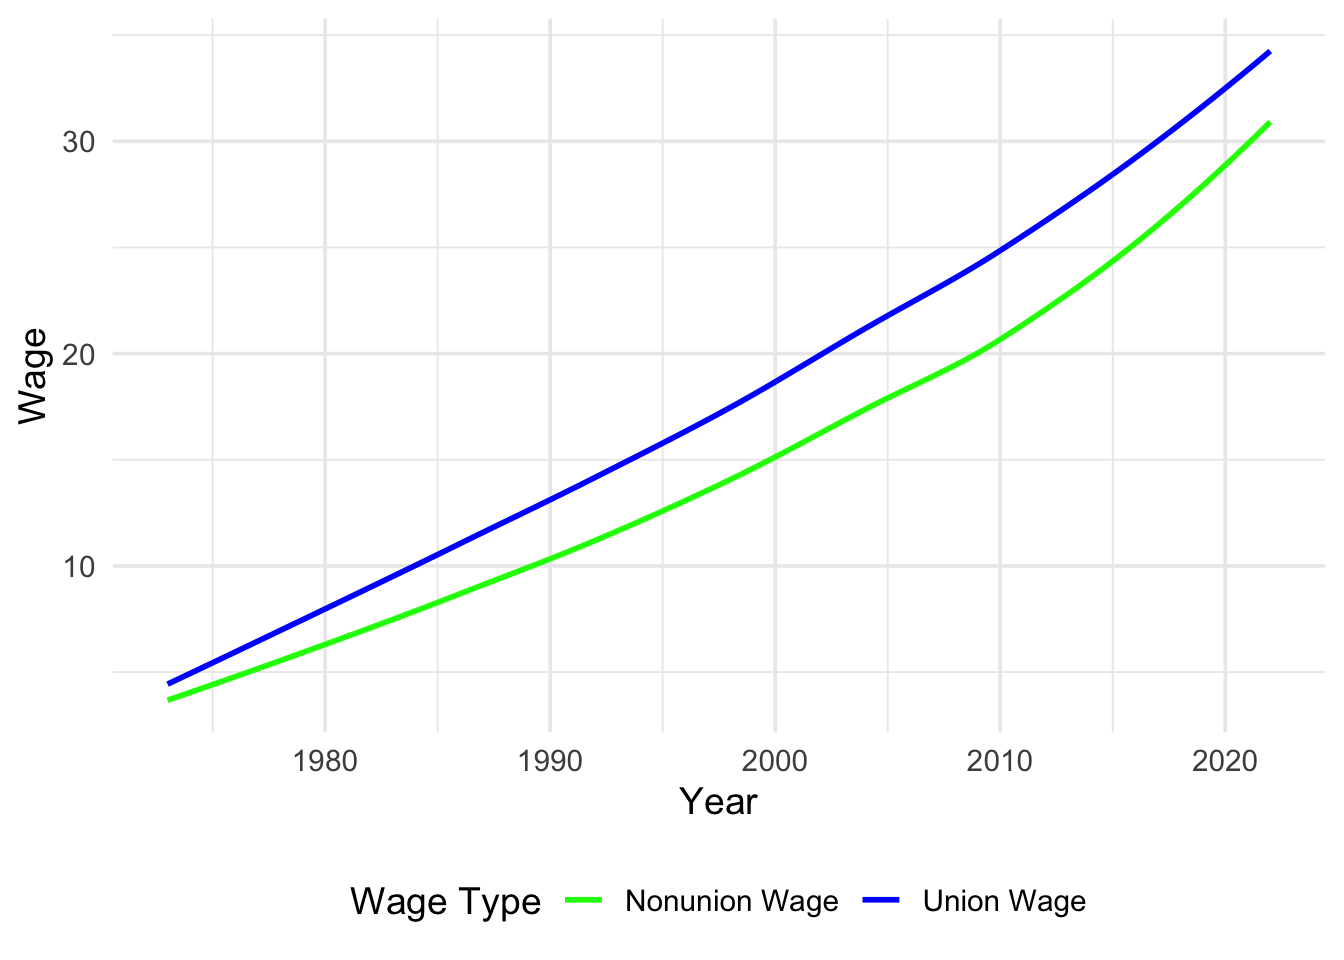
\includegraphics{_main_files/figure-latex/unnamed-chunk-18-1.pdf}
But it's not just about the money. Unions also fight for safer working conditions, better benefits like healthcare and paid time off, and they give workers a voice. Being part of a union means having real power to push back against unfair treatment and make sure you're getting what you need to thrive---not just survive. Lets focus just on earnings though.

\section{Recent Union Wins}\label{recent-union-wins}

\begin{itemize}
\item
  \textbf{Restoration of Salary Steps for California State University (CSU) Workers (2024):}\\
  Teamsters Local 2010 secured an agreement with CSU, reinstating a salary step system that had been absent for decades. The agreement included an immediate 5\% salary increase retroactive to July 1, 2023, and all members reaching their target salary step by July 2025.\citep{teamsters2024}
\item
  \textbf{United Auto Workers (UAW) Strike Achievements (2023):}\\
  In fall 2023, the UAW strike against major automakers resulted in substantial pay raises and improved working conditions. It was one of the most significant contract victories since the sit-down strikes of the 1930s. \citep{thenation2023}
\item
  \textbf{Unionization of Volkswagen's Chattanooga Plant (2024):}\\
  The UAW successfully unionized Volkswagen's Chattanooga, Tennessee, plant in April 2024. This was the first successful unionization at a foreign manufacturer's U.S. plant in the southern states. \citep{lemonde2024}
\item
  \textbf{Unionization of Blue Bird Bus Factory Workers (2023):}\\
  The United Steelworkers won an election at a Blue Bird bus factory in Georgia, unionizing nearly 1,500 predominantly Black workers in 2023.
\end{itemize}

\section{Unions are Growing!}\label{unions-are-growing}

As the economy changes so too does Union membership in certain job sectors. What your take away should be is that no matter the type of job you have, it can be unionized!

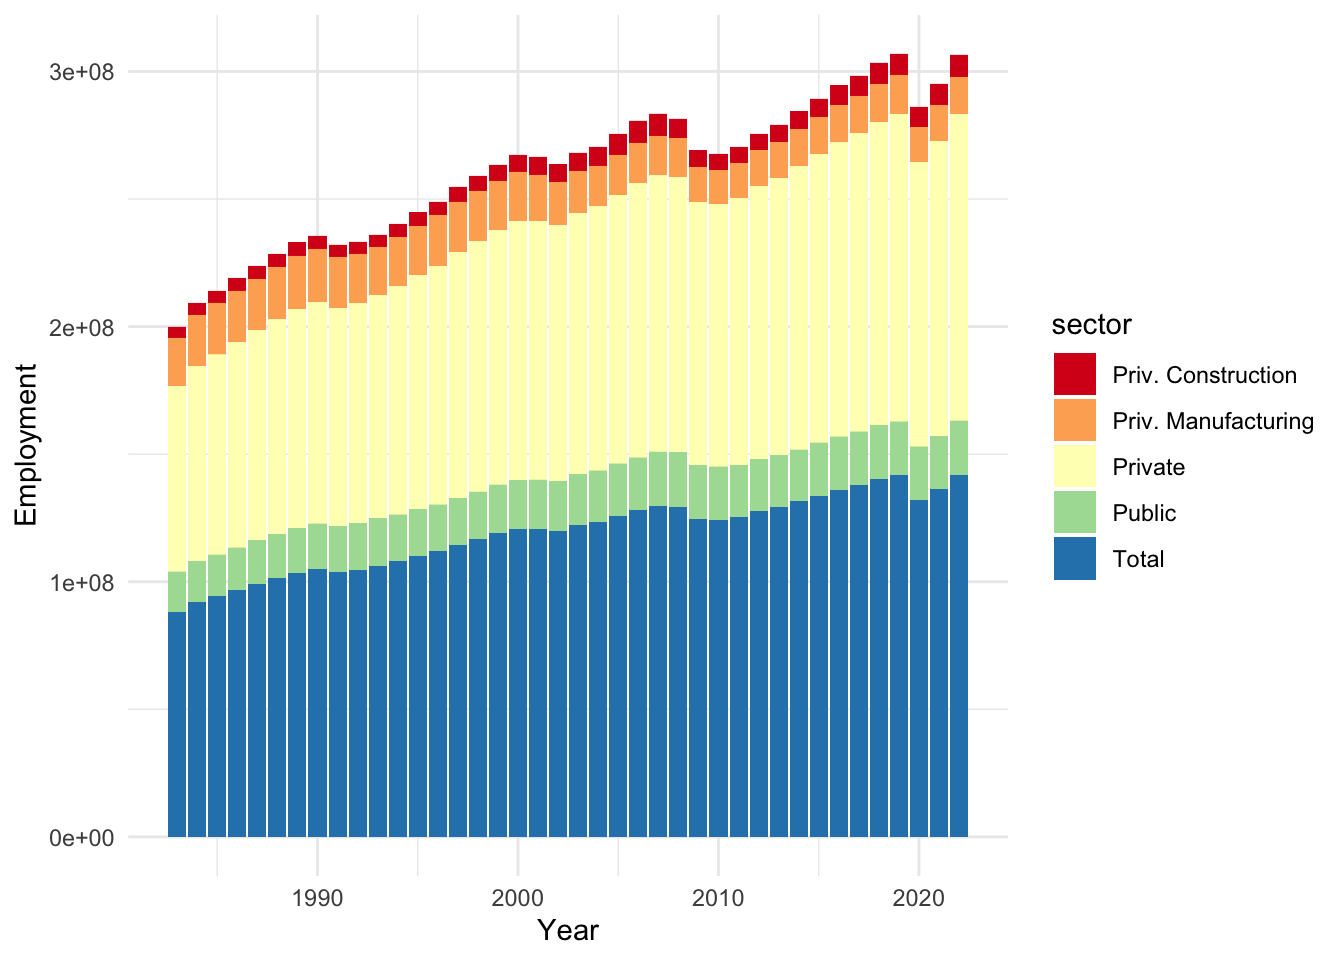
\includegraphics{_main_files/figure-latex/unnamed-chunk-19-1.pdf}

So join a union or start forming one of your own!

\section{Getting Involved!}\label{getting-involved}

\begin{itemize}
\tightlist
\item
  \textbf{Join a Union}: Check if there is an existing union that represents workers in your industry. The AFL-CIO website (\url{https://aflcio.org}) is a great starting point to find affiliated unions.
\item
  \textbf{Form a Union}: If there isn't one, consider forming your own. The National Labor Relations Board (\url{https://www.nlrb.gov}) provides resources to help workers understand their rights and the steps involved in unionizing.
\item
  \textbf{Connect with Organizers}: The United Electrical, Radio, and Machine Workers of America (UE) has guides on forming a union and can connect you with experienced organizers (\url{https://www.ueunion.org}).
\item
  \textbf{Get Educated}: Websites like Labor Notes (\url{https://labornotes.org}) offer valuable information about union organizing, labor rights, and how to take action.
\item
  \textbf{Reach Out to Local Chapters}: Look for local worker centers or community organizations that support unionization efforts. They can be a great source of advice and resources.
\item
  \textbf{Communication Workers of America (CWA)} -- CWA represents tech and telecommunications workers and has been actively organizing workers in the tech sector, including campaigns at Google and other tech companies. More information can be found here: \url{https://cwa-union.org}.
\end{itemize}

  \bibliography{book.bib}

\end{document}
